\documentclass{beamer}
\hypersetup{bookmarksdepth=5}

\usepackage[T1]{fontenc}   % required for luximono!
\usepackage{lmodern}
\usepackage[scaled=0.8]{luximono}  % typewriter font with bold face

% To install the luximono font files:
% getnonfreefonts-sys --all        or
% getnonfreefonts-sys luximono
%
% when there are trouble you might need to:
% - Create /etc/texmf/updmap.d/99local-luximono.cfg
%   containing the single line: Map ul9.map
% - Run update-updmap followed by mktexlsr and updmap-sys
%
% This commands must be executed as root with a root environment
% (i.e. run "sudo su" and then execute the commands in the root
% shell, don't just prefix the commands with "sudo").

% formats the text accourding the set language
\usepackage[english]{babel}
\usepackage{amsmath}
\usepackage{multirow}
\usepackage{booktabs}
\usepackage{listings}
\usepackage{setspace}
\usepackage{skull}
\usepackage{units}

\usepackage{tikz}
\usetikzlibrary{calc}
\usetikzlibrary{arrows}
\usetikzlibrary{scopes}
\usetikzlibrary{through}
\usetikzlibrary{shapes.geometric}

\lstset{basicstyle=\ttfamily}

\def\B#1{{\tt\textbackslash{}#1}}
\def\C#1{\lstinline[language=C++]{#1}}
\def\V#1{\lstinline[language=Verilog]{#1}}

\lstdefinelanguage{liberty}{
	morecomment=[s]{/*}{*/},
	morekeywords={library,cell,area,pin,direction,function,clocked_on,next_state,clock,ff},
	morestring=[b]",
}

\lstdefinelanguage{rtlil}{
	morecomment=[l]{\#},
	morekeywords={module,attribute,parameter,wire,memory,auto,width,offset,size,input,output,inout,cell,connect,switch,case,assign,sync,low,high,posedge,negedge,edge,always,update,process,end},
	morestring=[b]",
}

\lstdefinelanguage{ys}{
	morecomment=[l]{\#},
}

\lstset{
	commentstyle=\color{YosysGreen},
}

\newenvironment{boxalertenv}{\begin{altenv}%
{\usebeamertemplate{alerted text begin}\usebeamercolor[fg]{alerted text}\usebeamerfont{alerted text}\setlength{\fboxsep}{1pt}\colorbox{bg}}
{\usebeamertemplate{alerted text end}}{\color{.}}{}}{\end{altenv}}

\newcommand<>{\boxalert}[1]{{%
\begin{boxalertenv}#2{#1}\end{boxalertenv}%
}}

\newcommand{\subsectionpagesuffix}{
\vfill\begin{centering}
{\usebeamerfont{subsection name}\usebeamercolor[fg]{subsection name}of \sectionname~\insertsectionnumber}
\vskip1em\par
\setbeamercolor{graybox}{bg=gray}
\begin{beamercolorbox}[sep=8pt,center,bg=gray]{graybox}
\usebeamerfont{subsection title}\insertsection\par
\end{beamercolorbox}
\end{centering}}

\title{Yosys Open SYnthesis Suite}
\author{Clifford Wolf}
\institute{http://www.clifford.at/yosys/}

\usetheme{Madrid}
\usecolortheme{seagull}
\beamertemplatenavigationsymbolsempty

\definecolor{YosysGreen}{RGB}{85,136,102}
\definecolor{MyBlue}{RGB}{85,130,180}

\setbeamercolor{title}{fg=black,bg=YosysGreen!70}
\setbeamercolor{titlelike}{fg=black,bg=YosysGreen!70}
\setbeamercolor{frametitle}{fg=black,bg=YosysGreen!70}
\setbeamercolor{block title}{fg=black,bg=YosysGreen!70}
\setbeamercolor{item projected}{fg=black,bg=YosysGreen}

\begin{document}

\begin{frame}
\titlepage
\end{frame}

\setcounter{section}{-3}

\section{Abstract}
\begin{frame}{Abstract}
Yosys is the first full-featured open source software for Verilog HDL
synthesis. It supports most of Verilog-2005 and is well tested with
real-world designs from the ASIC and FPGA world.

\bigskip
Learn how to use Yosys to create your own custom synthesis flows and
discover why open source HDL synthesis is important for researchers,
hobbyists, educators and engineers alike.

\bigskip
This presentation covers basic concepts of Yosys, writing synthesis scripts
for a wide range of applications, creating Yosys scripts for various
non-synthesis applications (such as formal equivialence checking) and
writing extensions to Yosys using the C++ API.
\end{frame}

\section{About me}
\begin{frame}{About me}
Hi! I'm Clifford Wolf.

\bigskip
I like writing open source software. For example:
\begin{itemize}
\item Yosys
\item OpenSCAD (now maintained by Marius Kintel)
\item SPL (a not very popular scripting language)
\item EmbedVM (a very simple compiler+vm for 8 bit micros)
\item Lib(X)SVF (a library to play SVF/XSVF files over JTAG, used at LHC)
\item ROCK Linux (discontinued since 2010)
\end{itemize}
\end{frame}

\section{Outline}
\begin{frame}{Outline}
Yosys is an Open Source Verilog synthesis tool, and more.

\bigskip
Outline of this presentation:
\begin{itemize}
\item Introduction to the field and Yosys
\item Yosys by example: synthesis
\item Yosys by example: advanced synthesis
\item Yosys by example: beyond synthesis
\item Writing Yosys extensions in C++
\end{itemize}
\end{frame}


\section{Introduction}

\begin{frame}
\sectionpage
\end{frame}

%%%%%%%%%%%%%%%%%%%%%%%%%%%%%%%%%%%%%%%%%%%%%%%%%%%%%%%%%%%%%%%%%%%%%%%%%%%%%

\subsection{Representations of (digital) Circuits}

\begin{frame}[t]{\subsecname}
\begin{itemize}
	\item Graphical
		\begin{itemize}
			\item \alert<1>{Schematic Diagram}
			\item \alert<2>{Physical Layout}
		\end{itemize}
	\bigskip
	\item Non-graphical
		\begin{itemize}
			\item \alert<3>{Netlists}
			\item \alert<4>{Hardware Description Languages (HDLs)}
		\end{itemize}
\end{itemize}
\bigskip
\begin{block}{Definition:
\only<1>{Schematic Diagram}%
\only<2>{Physical Layout}%
\only<3>{Netlists}%
\only<4>{Hardware Description Languages (HDLs)}}
\only<1>{
	Graphical representation of the circtuit topology. Circuit elements
	are represented by symbols and electrical connections by lines. The gometric
	layout is for readability only.
}%
\only<2>{
	The actual physical geometry of the device (PCB or ASIC manufracturing masks).
	This is the final product of the design process.
}%
\only<3>{
	A list of circuit elements and a list of connections. This is the raw circuit
	topology.
}%
\only<4>{
	Computer languages (like programming languages) that can be used to describe
	circuits. HDLs are much more powerful in describing huge circuits than
	schematic diagrams.
}%
\end{block}
\end{frame}

%%%%%%%%%%%%%%%%%%%%%%%%%%%%%%%%%%%%%%%%%%%%%%%%%%%%%%%%%%%%%%%%%%%%%%%%%%%%%

\subsection{Levels of Abstraction for Digital Circuits}

\begin{frame}[t]{\subsecname}
\begin{itemize}
	\item \alert<1>{System Level}
	\item \alert<2>{High Level}
	\item \alert<3>{Behavioral Level}
	\item \alert<4>{Register-Transfer Level (RTL)}
	\item \alert<5>{Logical Gate Level}
	\item \alert<6>{Physical Gate Level}
	\item \alert<7>{Switch Level}
\end{itemize}
\bigskip
\begin{block}{Definition:
\only<1>{System Level}%
\only<2>{High Level}%
\only<3>{Behavioral Level}%
\only<4>{Register-Transfer Level (RTL)}%
\only<5>{Logical Gate Level}%
\only<6>{Physical Gate Level}%
\only<7>{Switch Level}}
\only<1>{
	Overall view of the circuit: E.g. block-diagrams or instruction-set architecture descriptions
}%
\only<2>{
	Functional implementation of circuit in high-level programming language (C, C++, SystemC, Matlab, Python, etc.).
}%
\only<3>{
	Cycle-accurate description of circuit in hardware description language (Verilog, VHDL, etc.).
}%
\only<4>{
	List of registers (flip-flops) and logic functions that calculate the next state from the previous one. Usually
	a netlist utilizing high-level cells such as adders, multiplieres, multiplexer, etc.
}%
\only<5>{
	Netlist of single-bit registers and basic logic gates (such as AND, OR,
	NOT, etc.). Popular form: And-Inverter-Graphs (AIGs) with pairs of primary
	inputs and outputs for each register bit.
}%
\only<6>{
	Netlist of cells that actually are available on the target architecture
	(such as CMOS gates in an ASCI or LUTs in an FPGA). Optimized for
	area and/or and/or speed (static timing or number of logic levels).
}%
\only<7>{
	Netlist of individual transistors.
}%
\end{block}
\end{frame}

%%%%%%%%%%%%%%%%%%%%%%%%%%%%%%%%%%%%%%%%%%%%%%%%%%%%%%%%%%%%%%%%%%%%%%%%%%%%%

\subsection{Digital Circuit Synthesis}

\begin{frame}{\subsecname}
	Synthesis Tools (such as Yosys) can transform HDL code to circuits:

	\bigskip
	\begin{center}
	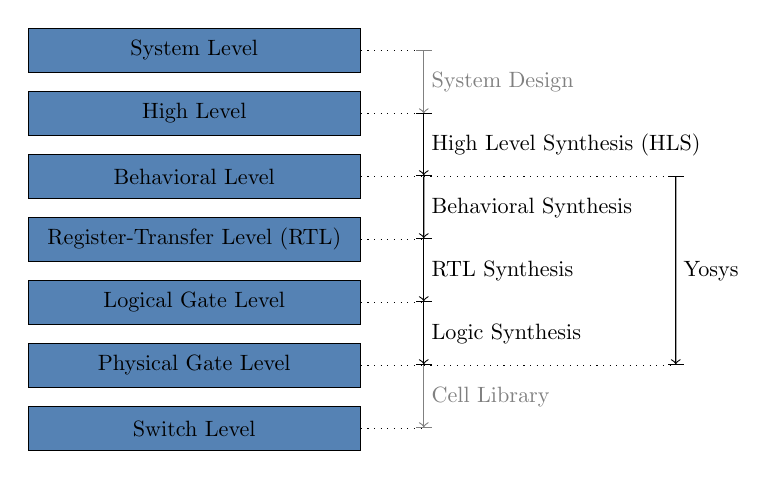
\begin{tikzpicture}[scale=0.8, every node/.style={transform shape}]
			\tikzstyle{lvl} = [draw, fill=MyBlue, rectangle, minimum height=2em, minimum width=15em]
			\node[lvl] (sys) {System Level};
			\node[lvl] (hl) [below of=sys] {High Level};
			\node[lvl] (beh) [below of=hl] {Behavioral Level};
			\node[lvl] (rtl) [below of=beh] {Register-Transfer Level (RTL)};
			\node[lvl] (lg) [below of=rtl] {Logical Gate Level};
			\node[lvl] (pg) [below of=lg] {Physical Gate Level};
			\node[lvl] (sw) [below of=pg] {Switch Level};

			\draw[dotted] (sys.east)  -- ++(1,0) coordinate (sysx);
			\draw[dotted] (hl.east)  -- ++(1,0) coordinate (hlx);
			\draw[dotted] (beh.east) -- ++(1,0) coordinate (behx);
			\draw[dotted] (rtl.east) -- ++(1,0) coordinate (rtlx);
			\draw[dotted] (lg.east)  -- ++(1,0) coordinate (lgx);
			\draw[dotted] (pg.east)  -- ++(1,0) coordinate (pgx);
			\draw[dotted] (sw.east)  -- ++(1,0) coordinate (swx);

			\draw[gray,|->] (sysx) -- node[right] {System Design} (hlx);
			\draw[|->|] (hlx) -- node[right] {High Level Synthesis (HLS)} (behx);
			\draw[->|] (behx) -- node[right] {Behavioral Synthesis} (rtlx);
			\draw[->|] (rtlx) -- node[right] {RTL Synthesis} (lgx);
			\draw[->|] (lgx) -- node[right] {Logic Synthesis} (pgx);
			\draw[gray,->|] (pgx) -- node[right] {Cell Library} (swx);

			\draw[dotted] (behx) -- ++(4,0) coordinate (a);
			\draw[dotted] (pgx) -- ++(4,0) coordinate (b);
			\draw[|->|] (a) -- node[right] {Yosys} (b);
	\end{tikzpicture}
	\end{center}
\end{frame}

%%%%%%%%%%%%%%%%%%%%%%%%%%%%%%%%%%%%%%%%%%%%%%%%%%%%%%%%%%%%%%%%%%%%%%%%%%%%%

\subsection{What Yosys can and can't do}

\begin{frame}{\subsecname}

Things Yosys can do:
\begin{itemize}
\item Read and process (most of) modern Verilog-2005 code.
\item Perform all kinds of operations on netlist (RTL, Logic, Gate).
\item Perform logic optimiziations and gate mapping with ABC\footnote[frame]{\url{http://www.eecs.berkeley.edu/~alanmi/abc/}}.
\end{itemize}

\bigskip
Things Yosys can't do:
\begin{itemize}
\item Process high-level languages such as C/C++/SystemC.
\item Create physical layouts (place\&route).
\end{itemize}

\bigskip
A typical flow combines Yosys with with a low-level implementation tool, such
as Qflow\footnote[frame]{\url{http://opencircuitdesign.com/qflow/}} for ASIC designs.

\end{frame}

%%%%%%%%%%%%%%%%%%%%%%%%%%%%%%%%%%%%%%%%%%%%%%%%%%%%%%%%%%%%%%%%%%%%%%%%%%%%%

\subsection{Yosys Data- and Control-Flow}

\begin{frame}{\subsecname}
	A (usually short) synthesis script controlls Yosys.

	This scripts contain three types of commands:
	\begin{itemize}
	\item {\bf Frontends}, that read input files (usually Verilog).
	\item {\bf Passes}, that perform transformation on the design in memory.
	\item {\bf Backends}, that write the design in memory to a file (various formats are available, e.g. Verilog, BLIF, EDIF, SPICE, BTOR, etc.).
	\end{itemize}

	\bigskip
	\begin{center}
	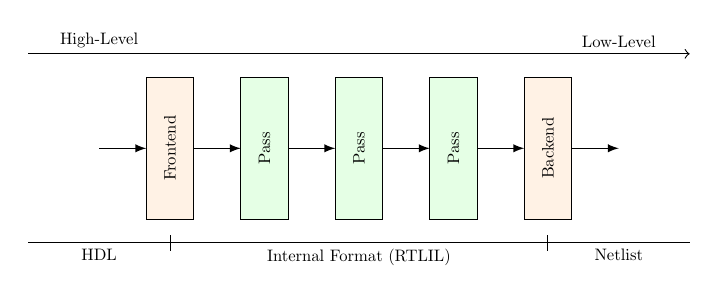
\begin{tikzpicture}[scale=0.6, every node/.style={transform shape}]
		\path (-1.5,3) coordinate (cursor);
		\draw[-latex] ($ (cursor) + (0,-1.5) $) -- ++(1,0);
		\draw[fill=orange!10] ($ (cursor) + (1,-3) $) rectangle node[rotate=90] {Frontend} ++(1,3) coordinate (cursor);
		\draw[-latex] ($ (cursor) + (0,-1.5) $) -- ++(1,0);
		\draw[fill=green!10] ($ (cursor) + (1,-3) $) rectangle node[rotate=90] {Pass} ++(1,3) coordinate (cursor);
		\draw[-latex] ($ (cursor) + (0,-1.5) $) -- ++(1,0);
		\draw[fill=green!10] ($ (cursor) + (1,-3) $) rectangle node[rotate=90] {Pass} ++(1,3) coordinate (cursor);
		\draw[-latex] ($ (cursor) + (0,-1.5) $) -- ++(1,0);
		\draw[fill=green!10] ($ (cursor) + (1,-3) $) rectangle node[rotate=90] {Pass} ++(1,3) coordinate (cursor);
		\draw[-latex] ($ (cursor) + (0,-1.5) $) -- ++(1,0);
		\draw[fill=orange!10] ($ (cursor) + (1,-3) $) rectangle node[rotate=90] {Backend} ++(1,3) coordinate (cursor);
		\draw[-latex] ($ (cursor) + (0,-1.5) $) -- ++(1,0);

		\path (-3,-0.5) coordinate (cursor);
		\draw (cursor) -- node[below] {HDL} ++(3,0) coordinate (cursor);
		\draw[|-|] (cursor) -- node[below] {Internal Format (RTLIL)} ++(8,0) coordinate (cursor);
		\draw (cursor) -- node[below] {Netlist} ++(3,0);

		\path (-3,3.5) coordinate (cursor);
		\draw[-] (cursor) -- node[above] {High-Level} ++(3,0) coordinate (cursor);
		\draw[-] (cursor) -- ++(8,0) coordinate (cursor);
		\draw[->] (cursor) -- node[above] {Low-Level} ++(3,0);
	\end{tikzpicture}
	\end{center}
\end{frame}

%%%%%%%%%%%%%%%%%%%%%%%%%%%%%%%%%%%%%%%%%%%%%%%%%%%%%%%%%%%%%%%%%%%%%%%%%%%%%

\subsection{Program Components and Data Formats}

\begin{frame}{\subsecname}
	\begin{center}
	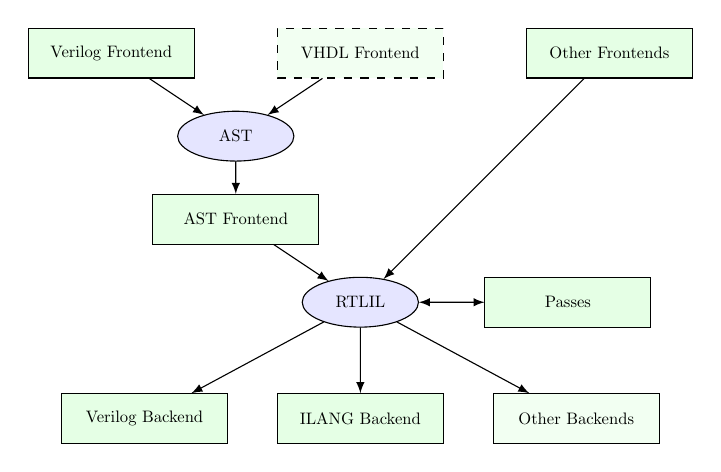
\begin{tikzpicture}[scale=0.6, every node/.style={transform shape}]
		\tikzstyle{process} = [draw, fill=green!10, rectangle, minimum height=3em, minimum width=10em, node distance=15em]
		\tikzstyle{data} = [draw, fill=blue!10, ellipse, minimum height=3em, minimum width=7em, node distance=15em]
		\node[process] (vlog) {Verilog Frontend};
		\node[process, dashed, fill=green!5] (vhdl) [right of=vlog] {VHDL Frontend};
		\node[process] (ilang) [right of=vhdl] {Other Frontends};
		\node[data] (ast) [below of=vlog, node distance=5em, xshift=7.5em] {AST};
		\node[process] (astfe) [below of=ast, node distance=5em] {AST Frontend};
		\node[data] (rtlil) [below of=astfe, node distance=5em, xshift=7.5em] {RTLIL};
		\node[process] (pass) [right of=rtlil, node distance=5em, xshift=7.5em] {Passes};
		\node[process] (vlbe) [below of=rtlil, node distance=7em, xshift=-13em] {Verilog Backend};
		\node[process] (ilangbe) [below of=rtlil, node distance=7em, xshift=0em] {ILANG Backend};
		\node[process, fill=green!5] (otherbe) [below of=rtlil, node distance=7em, xshift=+13em] {Other Backends};

		\draw[-latex] (vlog) -- (ast);
		\draw[-latex] (vhdl) -- (ast);
		\draw[-latex] (ast) -- (astfe);
		\draw[-latex] (astfe) -- (rtlil);
		\draw[-latex] (ilang) -- (rtlil);
		\draw[latex-latex] (rtlil) -- (pass);
		\draw[-latex] (rtlil) -- (vlbe);
		\draw[-latex] (rtlil) -- (ilangbe);
		\draw[-latex] (rtlil) -- (otherbe);
	\end{tikzpicture}
	\end{center}
\end{frame}

%%%%%%%%%%%%%%%%%%%%%%%%%%%%%%%%%%%%%%%%%%%%%%%%%%%%%%%%%%%%%%%%%%%%%%%%%%%%%

\subsection{Example Problem}

\begin{frame}[fragile]{\subsecname{} -- Verilog Source: \tt counter.v}
\lstinputlisting[xleftmargin=1cm, language=Verilog]{PRESENTATION_Intro/counter.v}
\end{frame}

\begin{frame}[fragile]{\subsecname{} -- Cell Library: \tt mycells.lib}
\begin{columns}
\column[t]{5cm}
\lstinputlisting[basicstyle=\ttfamily\fontsize{8pt}{10pt}\selectfont, language=liberty, lastline=20]{PRESENTATION_Intro/mycells.lib}
\column[t]{5cm}
\lstinputlisting[basicstyle=\ttfamily\fontsize{8pt}{10pt}\selectfont, language=liberty, firstline=21]{PRESENTATION_Intro/mycells.lib}
\end{columns}
\end{frame}

%%%%%%%%%%%%%%%%%%%%%%%%%%%%%%%%%%%%%%%%%%%%%%%%%%%%%%%%%%%%%%%%%%%%%%%%%%%%%

\subsection{Example Synthesis Script}

\begin{frame}[t]{\subsecname}

\setbeamercolor{alerted text}{fg=white,bg=red}

\begin{minipage}[t]{6cm}
\tt\scriptsize
\# read design\\
\boxalert<1>{read\_verilog counter.v}\\
\boxalert<2>{hierarchy -check -top counter}

\medskip
\# the high-level stuff\\
\boxalert<3>{proc}; \boxalert<4>{opt}; \boxalert<5>{memory}; \boxalert<6>{opt}; \boxalert<7>{fsm}; \boxalert<8>{opt}

\medskip
\# mapping to internal cell library\\
\boxalert<9>{techmap}; \boxalert<10>{opt}

\bigskip
\it continued\dots
\end{minipage}
\begin{minipage}[t]{5cm}
\tt\scriptsize
\# mapping flip-flops to mycells.lib\\
\boxalert<11>{dfflibmap -liberty mycells.lib}

\medskip
\# mapping logic to mycells.lib\\
\boxalert<12>{abc -liberty mycells.lib}

\medskip
\# cleanup\\
\boxalert<13>{clean}

\medskip
\# write synthesized design\\
\boxalert<14>{write\_verilog synth.v}
\end{minipage}

\vskip1cm

\begin{block}{Command: \tt
\only<1>{read\_verilog counter.v}%
\only<2>{hierarchy -check -top counter}%
\only<3>{proc}%
\only<4>{opt}%
\only<5>{memory}%
\only<6>{opt}%
\only<7>{fsm}%
\only<8>{opt}%
\only<9>{techmap}%
\only<10>{opt}%
\only<11>{dfflibmap -liberty mycells.lib}%
\only<12>{abc -liberty mycells.lib}%
\only<13>{clean}%
\only<14>{write\_verilog synth.v}}
\only<1>{
	Read Verilog source file and convert to internal representation.
}%
\only<2>{
	Elaborate the design hierarchy. Should alsways be the first
	command after reading the design.
}%
\only<3>{
	Convert ``processes'' (the internal representation of behavioral
	Verilog code) into multiplexers and registers.
}%
\only<4>{
	Perform some basic optimizations and cleanups.
}%
\only<5>{
	Analyze memories and create circuits to implement them.
}%
\only<6>{
	Perform some basic optimizations and cleanups.
}%
\only<7>{
	Analyze and optimize finite state machines.
}%
\only<8>{
	Perform some basic optimizations and cleanups.
}%
\only<9>{
	Map coarse-grain RTL cells (adders, etc.) to fine-grain
	logic gates (AND, OR, NOT, etc.).
}%
\only<10>{
	Perform some basic optimizations and cleanups.
}%
\only<11>{
	Map registers to available hardware flip-flops.
}%
\only<12>{
	Map logix to available hardware gates.
}%
\only<13>{
	Clean up the design (just the last step of {\tt opt}).
}%
\only<14>{
	Write final synthesis result to output file.
}%
\end{block}

\end{frame}

%%%%%%%%%%%%%%%%%%%%%%%%%%%%%%%%%%%%%%%%%%%%%%%%%%%%%%%%%%%%%%%%%%%%%%%%%%%%%

\subsection{Running the Synthesis Script}

\begin{frame}[t, fragile]{\subsecname{} -- Step 1/4}
\begin{verbatim}
read_verilog counter.v
hierarchy -check -top counter
\end{verbatim}

\vfill
\includegraphics[width=\linewidth,trim=0 0cm 0 0cm]{PRESENTATION_Intro/counter_00.pdf}
\end{frame}

\begin{frame}[t, fragile]{\subsecname{} -- Step 2/4}
\begin{verbatim}
proc; opt; memory; opt; fsm; opt
\end{verbatim}

\vfill
\includegraphics[width=\linewidth,trim=0 0cm 0 0cm]{PRESENTATION_Intro/counter_01.pdf}
\end{frame}

\begin{frame}[t, fragile]{\subsecname{} -- Step 3/4}
\begin{verbatim}
techmap; opt
\end{verbatim}

\vfill
\includegraphics[width=\linewidth,trim=0 0cm 0 0cm]{PRESENTATION_Intro/counter_02.pdf}
\end{frame}

\begin{frame}[t, fragile]{\subsecname{} -- Step 4/4}
\begin{verbatim}
dfflibmap -liberty mycells.lib
abc -liberty mycells.lib
clean
\end{verbatim}

\vfill
\includegraphics[width=\linewidth,trim=0 0cm 0 0cm]{PRESENTATION_Intro/counter_03.pdf}
\end{frame}

%%%%%%%%%%%%%%%%%%%%%%%%%%%%%%%%%%%%%%%%%%%%%%%%%%%%%%%%%%%%%%%%%%%%%%%%%%%%%

\subsection{Yosys Commands}

\begin{frame}[fragile]{\subsecname{} 1/3 \hspace{0pt plus 1 filll} (excerpt)}
Command reference:
\begin{itemize}
\item Use ``{\tt help}'' for a command list and ``{\tt help \it command}'' for details.
\item Or run ``{\tt yosys -H}'' and ``{\tt yosys -h \it command}''.
\item Or go to \url{http://www.clifford.at/yosys/documentation.html}.
\end{itemize}

\bigskip
Commands for design navigation and investigation:
\begin{lstlisting}[xleftmargin=1cm, basicstyle=\ttfamily\fontsize{8pt}{10pt}\selectfont]
    cd                   a shortcut for 'select -module <name>'
    ls                   list modules or objects in modules
    dump                 print parts of the design in ilang format
    show                 generate schematics using graphviz
    select               modify and view the list of selected objects
\end{lstlisting}

\bigskip
Commands for executing scripts or entering interactive mode:
\begin{lstlisting}[xleftmargin=1cm, basicstyle=\ttfamily\fontsize{8pt}{10pt}\selectfont]
    shell                enter interactive command mode
    history              show last interactive commands
    script               execute commands from script file
    tcl                  execute a TCL script file
\end{lstlisting}
\end{frame}

\begin{frame}[fragile]{\subsecname{} 2/3 \hspace{0pt plus 1 filll} (excerpt)}
Commands for reading and elaborating the design:
\begin{lstlisting}[xleftmargin=1cm, basicstyle=\ttfamily\fontsize{8pt}{10pt}\selectfont]
    read_ilang           read modules from ilang file
    read_verilog         read modules from verilog file
    hierarchy            check, expand and clean up design hierarchy
\end{lstlisting}

\bigskip
Commands for high-level synthesis:
\begin{lstlisting}[xleftmargin=1cm, basicstyle=\ttfamily\fontsize{8pt}{10pt}\selectfont]
    proc                 translate processes to netlists
    fsm                  extract and optimize finite state machines
    memory               translate memories to basic cells
    opt                  perform simple optimizations
\end{lstlisting}

\bigskip
Commands for technology mapping:
\begin{lstlisting}[xleftmargin=1cm, basicstyle=\ttfamily\fontsize{8pt}{10pt}\selectfont]
    techmap              simple technology mapper
    abc                  use ABC for technology mapping
    dfflibmap            technology mapping of flip-flops
    hilomap              technology mapping of constant hi- and/or lo-drivers
    iopadmap             technology mapping of i/o pads (or buffers)
    flatten              flatten design
\end{lstlisting}
\end{frame}

\begin{frame}[fragile]{\subsecname{} 3/3 \hspace{0pt plus 1 filll} (excerpt)}
Commands for writing the results:
\begin{lstlisting}[xleftmargin=1cm, basicstyle=\ttfamily\fontsize{8pt}{10pt}\selectfont]
    write_blif           write design to BLIF file
    write_btor           write design to BTOR file
    write_edif           write design to EDIF netlist file
    write_ilang          write design to ilang file
    write_spice          write design to SPICE netlist file
    write_verilog        write design to verilog file
\end{lstlisting}

\bigskip
Script-Commands for standard synthesis tasks:
\begin{lstlisting}[xleftmargin=1cm, basicstyle=\ttfamily\fontsize{8pt}{10pt}\selectfont]
    synth_xilinx         synthesis for Xilinx FPGAs
\end{lstlisting}

\bigskip
... and many many more.
\end{frame}

%%%%%%%%%%%%%%%%%%%%%%%%%%%%%%%%%%%%%%%%%%%%%%%%%%%%%%%%%%%%%%%%%%%%%%%%%%%%%

\subsection{More Verilog Examples}

\begin{frame}[fragile]{\subsecname{} 1/3}
\begin{lstlisting}[xleftmargin=1cm, basicstyle=\ttfamily\fontsize{8pt}{10pt}\selectfont, language=Verilog]
module detectprime(a, y);
    input [4:0] a;
    output y;

    integer i, j;
    reg [31:0] lut;

    initial begin
        for (i = 0; i < 32; i = i+1) begin
            lut[i] = i > 1;
            for (j = 2; j*j <= i; j = j+1)
                if (i % j == 0)
                    lut[i] = 0;
        end
    end

    assign y = lut[a];
endmodule
\end{lstlisting}
\end{frame}

\begin{frame}[fragile]{\subsecname{} 2/3}
\begin{lstlisting}[xleftmargin=1cm, basicstyle=\ttfamily\fontsize{8pt}{10pt}\selectfont, language=Verilog]
module carryadd(a, b, y);
    parameter WIDTH = 8;
    input [WIDTH-1:0] a, b;
    output [WIDTH-1:0] y;

    genvar i;
    generate
        for (i = 0; i < WIDTH; i = i+1) begin:STAGE
            wire IN1 = a[i], IN2 = b[i];
            wire C, Y;
            if (i == 0)
                assign C = IN1 & IN2, Y = IN1 ^ IN2;
            else
                assign C = (IN1 & IN2) | ((IN1 | IN2) & STAGE[i-1].C),
                       Y = IN1 ^ IN2 ^ STAGE[i-1].C;
            assign y[i] = Y;
        end
    endgenerate
endmodule
\end{lstlisting}
\end{frame}

\begin{frame}[fragile]{\subsecname{} 3/3}
\begin{lstlisting}[xleftmargin=1cm, basicstyle=\ttfamily\fontsize{7pt}{8.5pt}\selectfont, language=Verilog]
module cam(clk, wr_enable, wr_addr, wr_data, rd_data, rd_addr, rd_match);
    parameter WIDTH = 8;
    parameter DEPTH = 16;
    localparam ADDR_BITS = $clog2(DEPTH);

    input clk, wr_enable;
    input [ADDR_BITS-1:0] wr_addr;
    input [WIDTH-1:0] wr_data, rd_data;
    output reg [ADDR_BITS-1:0] rd_addr;
    output reg rd_match;

    integer i;
    reg [WIDTH-1:0] mem [0:DEPTH-1];

    always @(posedge clk) begin
        rd_addr <= 'bx;
        rd_match <= 0;
        for (i = 0; i < DEPTH; i = i+1)
            if (mem[i] == rd_data) begin
                rd_addr <= i;
                rd_match <= 1;
            end
        if (wr_enable)
            mem[wr_addr] <= wr_data;
    end
endmodule
\end{lstlisting}
\end{frame}

\subsection{Verification}

\begin{frame}{\subsecname}
Contiously checking the correctness of Yosys and making sure that new features
do not break old ones is a high priority in Yosys.

\bigskip
There are two external test suites build for Yosys: VlogHammer and yosys-bigsim
(see next slides)

\bigskip
In addition to that, yosys comes with $\approx\!200$ test cases used in ``{\tt make test}''.

\bigskip
A debug build of Yosys also contains a lot of asserts and checks the integrity of
the internal state after each command.
\end{frame}

\begin{frame}[fragile]{\subsecname{} -- VlogHammer}
VlogHammer is a Verilog regression test suite developed to test the different
subsystems in Yosys by comparing them to each other and the implementations
generated by some proprietary tools (Xilinx Vivado, Xilinx XST, Altera Quartus II, ...).

\bigskip
Yosys Subsystems tested: Verilog frontend, const folding, const eval, technology mapping,
simulation models, SAT models.

\bigskip
Thousands of auto-generated test cases containing code such as:
\begin{lstlisting}[xleftmargin=1cm, basicstyle=\ttfamily\fontsize{8pt}{10pt}\selectfont, language=Verilog]
assign y9 = $signed(((+$signed((^(6'd2 ** a2))))<$unsigned($unsigned(((+a3))))));
assign y10 = (-((+((+{2{(~^p13)}})))^~(!{{b5,b1,a0},(a1&p12),(a4+a3)})));
assign y11 = (~&(-{(-3'sd3),($unsigned($signed($unsigned({p0,b4,b1}))))}));
\end{lstlisting}

\bigskip
Some bugs in Yosys where found and fixed thanks to VlogHammer. Over 20 bugs in
the proprietary tools used as external reference where found and reported.
\end{frame}

\begin{frame}{\subsecname{} -- yosys-bigsim}
yosys-bigsim is a collection of real-world open-source Verilog designs and test
benches. yosys-bigsim compares the testbench outpus of simulations of the original
Verilog code and synthesis results.

\bigskip
The following designs are part of yosys-bigsim:
\begin{itemize}
\item {\tt openmsp430} -- an MSP430 compatible 16 bit CPU
\item {\tt aes\_5cycle\_2stage} -- an AES encryption core
\item {\tt softusb\_navre} -- an AVR compatible 8 bit CPU
\item {\tt amber23} -- an ARMv2 compatible 32 bit CPU
\item {\tt lm32} -- another 32 bit CPU from Lattice Semiconductor
\item {\tt verilog-pong} -- a hardware pong game with VGA output
\item {\tt elliptic\_curve\_group} -- ECG point-add and point-scalar-mul core
\item {\tt reed\_solomon\_decoder} -- a Reed-Solomon Error Correction Decoder
\end{itemize}
\end{frame}

%%%%%%%%%%%%%%%%%%%%%%%%%%%%%%%%%%%%%%%%%%%%%%%%%%%%%%%%%%%%%%%%%%%%%%%%%%%%%

\subsection{Benefits of Open Source HDL Synthesis}

\begin{frame}{\subsecname{} -- 1/3}
\begin{itemize}
\item Cost (also applies to ``free as in free beer'' solutions): \smallskip\par
Today the cost for a mask set in $\unit[180]{nm}$ technology is far less than
the cost for the design tools needed to design the mask layouts. Open Source
ASIC flows are an important enabler for ASIC-level Open Source Hardware.

\bigskip
\item Availablity and Reproducability: \smallskip\par
If you are a researcher who is publishing, you want to use tools that everyone
else can also use. Even if most universities have access to all major
commercial tools, you usually do not have easy access to the version that was
used in a research project a couple of years ago. With Open Source tools you
can even release the source code of the tool you have used alongside your data.
\end{itemize}
\end{frame}

\begin{frame}{\subsecname{} -- 2/3}
\begin{itemize}
\item Framework: \smallskip\par
Yosys is not only a tool. It is a framework that can be used as basis for other
developments, so researchers and hackers alike do not need to re-invent the
basic functionality. Extensibility was one of Yosys' design goals.

\bigskip
\item All-in-one: \smallskip\par
Because of the framework characterisitcs of Yosys, an increasing number of features
become available in one tool. Yosys not only can be used for circuit synthesis but
also for formal equivialence checking, SAT solving, and for circuit analysis, to
name just a few other application domains. With propritaery software one needs to
learn a new tool for each of this applications.
\end{itemize}
\end{frame}

\begin{frame}{\subsecname{} -- 3/3}
\begin{itemize}
\item Educational Tool: \smallskip\par
Propritaery synthesis tools are at times where secretive about their inner
workings. They often are ``black boxes'' where a design goes in and synthesis
results come out. Yosys is very open about its internals and it is easy to
observe the different steps of synthesis.
\end{itemize}

\bigskip
\begin{block}{BTW: Yosys is licensed under the ISC license:}
Permission to use, copy, modify, and/or distribute this software for any
purpose with or without fee is hereby granted, provided that the above
copyright notice and this permission notice appear in all copies.
\end{block}
\end{frame}

%%%%%%%%%%%%%%%%%%%%%%%%%%%%%%%%%%%%%%%%%%%%%%%%%%%%%%%%%%%%%%%%%%%%%%%%%%%%%



\section{Yosys by example -- Synthesis}

\begin{frame}
\sectionpage
\end{frame}

%%%%%%%%%%%%%%%%%%%%%%%%%%%%%%%%%%%%%%%%%%%%%%%%%%%%%%%%%%%%%%%%%%%%%%%%%%%%%

\subsection{Typical Phases of a Synthesis Flow}

\begin{frame}{\subsecname}
\begin{itemize}
\item Reading and elaborating the design
\item High-level synthesis and optimization
\begin{itemize}
\item Converting {\tt always}-blocks to logic and registers
\item Perform coarse-grain optimizations (resource sharing, const folding, ...)
\item Handling of memories and other coarse-grain blocks
\item Extracting and optimizing finite state machines
\end{itemize}
\item Convert remaining logic to bit-level logic functions
\item Perform optimizations on bit-level logic functions
\item Map bit-level logic and register to gates from cell library
\item Write results to output file 
\end{itemize}
\end{frame}

%%%%%%%%%%%%%%%%%%%%%%%%%%%%%%%%%%%%%%%%%%%%%%%%%%%%%%%%%%%%%%%%%%%%%%%%%%%%%

\subsection{Reading the design}

\begin{frame}[fragile]{\subsecname}
\begin{lstlisting}[xleftmargin=0.5cm, basicstyle=\ttfamily\fontsize{8pt}{10pt}\selectfont]
read_verilog file1.v
read_verilog -I include_dir -D enable_foo -D WIDTH=12 file2.v
read_verilog -lib cell_library.v

verilog_defaults -add -I include_dir
read_verilog file3.v
read_verilog file4.v
verilog_defaults -clear

verilog_defaults -push
verilog_defaults -add -I include_dir
read_verilog file5.v
read_verilog file6.v
verilog_defaults -pop
\end{lstlisting}
\end{frame}

%%%%%%%%%%%%%%%%%%%%%%%%%%%%%%%%%%%%%%%%%%%%%%%%%%%%%%%%%%%%%%%%%%%%%%%%%%%%%

\subsection{Design elaboration}

\begin{frame}[fragile]{\subsecname}
During design elaboration Yosys figures out how the modules are hierarchically
connected. It also re-runs the AST parts of the Verilog frontend to create
all needed variations of parametric modules.

\bigskip
\begin{lstlisting}[xleftmargin=0.5cm, basicstyle=\ttfamily\fontsize{8pt}{10pt}\selectfont]
# simplest form. at least this version should be used after reading all input files
#
hierarchy

# recommended form. fail if parts of the design hierarchy are missing. remove
# everything that is unreachable by the top module. mark the top module.
#
hierarchy -check -top top_module
\end{lstlisting}
\end{frame}

%%%%%%%%%%%%%%%%%%%%%%%%%%%%%%%%%%%%%%%%%%%%%%%%%%%%%%%%%%%%%%%%%%%%%%%%%%%%%

\subsection{The ``proc'' commands}

\begin{frame}[fragile]{\subsecname}
The Verilog frontend converts {\tt always}-blocks to RTL netlists for the
expressions and ``processes'' for the control- and memory elements.

\medskip
The {\tt proc} command transforms this ``processes'' to netlists of RTL
multiplexer and register cells.

\medskip
The {\tt proc} command is actually a macro-command that calls the following
other commands:

\begin{lstlisting}[xleftmargin=0.5cm, basicstyle=\ttfamily\fontsize{8pt}{10pt}\selectfont]
proc_clean      # remove empty branches and processes
proc_rmdead     # remove unreachable branches
proc_init       # special handling of "initial" blocks
proc_arst       # identify modeling of async resets
proc_mux        # convert decision trees to multiplexer networks
proc_dff        # extract registers from processes
proc_clean      # if all went fine, this should remove all the processes
\end{lstlisting}

\medskip
Many commands can not operate on modules with ``processes'' in them. Usually
a call to {\tt proc} is the first command in the actual synthesis procedure
after design elaboration.
\end{frame}

\begin{frame}[fragile]{\subsecname{} -- Example 1/3}
\begin{columns}
\column[t]{5cm}
\lstinputlisting[basicstyle=\ttfamily\fontsize{8pt}{10pt}\selectfont, language=verilog]{PRESENTATION_ExSyn/proc_01.v}
\column[t]{5cm}
\lstinputlisting[basicstyle=\ttfamily\fontsize{8pt}{10pt}\selectfont, frame=single]{PRESENTATION_ExSyn/proc_01.ys}
\end{columns}
\hfil\includegraphics[width=8cm,trim=0 0cm 0 0cm]{PRESENTATION_ExSyn/proc_01.pdf}
\end{frame}

\begin{frame}[t, fragile]{\subsecname{} -- Example 2/3}
\vbox to 0cm{\includegraphics[width=\linewidth,trim=0cm 0cm 0cm -2.5cm]{PRESENTATION_ExSyn/proc_02.pdf}\vss}
\vskip-1cm
\begin{columns}
\column[t]{5cm}
\lstinputlisting[basicstyle=\ttfamily\fontsize{8pt}{10pt}\selectfont, language=verilog]{PRESENTATION_ExSyn/proc_02.v}
\column[t]{5cm}
\lstinputlisting[basicstyle=\ttfamily\fontsize{8pt}{10pt}\selectfont, frame=single]{PRESENTATION_ExSyn/proc_02.ys}
\end{columns}
\end{frame}

\begin{frame}[t, fragile]{\subsecname{} -- Example 3/3}
\vbox to 0cm{\includegraphics[width=\linewidth,trim=0cm 0cm 0cm -1.5cm]{PRESENTATION_ExSyn/proc_03.pdf}\vss}
\vskip-1cm
\begin{columns}
\column[t]{5cm}
\lstinputlisting[basicstyle=\ttfamily\fontsize{8pt}{10pt}\selectfont, frame=single]{PRESENTATION_ExSyn/proc_03.ys}
\column[t]{5cm}
\lstinputlisting[basicstyle=\ttfamily\fontsize{8pt}{10pt}\selectfont, language=verilog]{PRESENTATION_ExSyn/proc_03.v}
\end{columns}
\end{frame}

%%%%%%%%%%%%%%%%%%%%%%%%%%%%%%%%%%%%%%%%%%%%%%%%%%%%%%%%%%%%%%%%%%%%%%%%%%%%%

\subsection{The ``opt'' commands}

\begin{frame}[fragile]{\subsecname}
The {\tt opt} command implements a series of simple optimizations. It also
is a macro command that calls other commands:

\begin{lstlisting}[xleftmargin=0.5cm, basicstyle=\ttfamily\fontsize{8pt}{10pt}\selectfont]
opt_const               # const folding
opt_share -nomux        # merging identical cells

do
    opt_muxtree         # remove never-active branches from multiplexer tree
    opt_reduce          # consolidate trees of boolean ops to reduce functions
    opt_share           # merging identical cells
    opt_rmdff           # remove/simplify registers with constant inputs
    opt_clean           # remove unused objects (cells, wires) from design
    opt_const           # const folding
while [changed design]
\end{lstlisting}

The command {\tt clean} can be used as alias for {\tt opt\_clean}. And {\tt ;;}
can be used as shortcut for {\tt clean}. For example:

\begin{lstlisting}[xleftmargin=0.5cm, basicstyle=\ttfamily\fontsize{8pt}{10pt}\selectfont]
proc; opt; memory; opt_const;; fsm;;
\end{lstlisting}
\end{frame}

\begin{frame}[t, fragile]{\subsecname{} -- Example 1/4}
\vbox to 0cm{\includegraphics[width=\linewidth,trim=0cm 0cm 0cm -0.5cm]{PRESENTATION_ExSyn/opt_01.pdf}\vss}
\vskip-1cm
\begin{columns}
\column[t]{5cm}
\lstinputlisting[basicstyle=\ttfamily\fontsize{8pt}{10pt}\selectfont, frame=single]{PRESENTATION_ExSyn/opt_01.ys}
\column[t]{5cm}
\lstinputlisting[basicstyle=\ttfamily\fontsize{8pt}{10pt}\selectfont, language=verilog]{PRESENTATION_ExSyn/opt_01.v}
\end{columns}
\end{frame}

\begin{frame}[t, fragile]{\subsecname{} -- Example 2/4}
\vbox to 0cm{\includegraphics[width=\linewidth,trim=0cm 0cm 0cm 0cm]{PRESENTATION_ExSyn/opt_02.pdf}\vss}
\vskip-1cm
\begin{columns}
\column[t]{5cm}
\lstinputlisting[basicstyle=\ttfamily\fontsize{8pt}{10pt}\selectfont, frame=single]{PRESENTATION_ExSyn/opt_02.ys}
\column[t]{5cm}
\lstinputlisting[basicstyle=\ttfamily\fontsize{8pt}{10pt}\selectfont, language=verilog]{PRESENTATION_ExSyn/opt_02.v}
\end{columns}
\end{frame}

\begin{frame}[t, fragile]{\subsecname{} -- Example 3/4}
\vbox to 0cm{\includegraphics[width=\linewidth,trim=0cm 0cm 0cm -2cm]{PRESENTATION_ExSyn/opt_03.pdf}\vss}
\vskip-1cm
\begin{columns}
\column[t]{5cm}
\lstinputlisting[basicstyle=\ttfamily\fontsize{8pt}{10pt}\selectfont, frame=single]{PRESENTATION_ExSyn/opt_03.ys}
\column[t]{5cm}
\lstinputlisting[basicstyle=\ttfamily\fontsize{8pt}{10pt}\selectfont, language=verilog]{PRESENTATION_ExSyn/opt_03.v}
\end{columns}
\end{frame}

\begin{frame}[t, fragile]{\subsecname{} -- Example 4/4}
\vbox to 0cm{\hskip6cm\includegraphics[width=6cm,trim=0cm 0cm 0cm -3cm]{PRESENTATION_ExSyn/opt_04.pdf}\vss}
\vskip-1cm
\begin{columns}
\column[t]{5cm}
\lstinputlisting[basicstyle=\ttfamily\fontsize{8pt}{10pt}\selectfont, language=verilog]{PRESENTATION_ExSyn/opt_04.v}
\column[t]{5cm}
\lstinputlisting[basicstyle=\ttfamily\fontsize{8pt}{10pt}\selectfont, frame=single]{PRESENTATION_ExSyn/opt_04.ys}
\end{columns}
\end{frame}

%%%%%%%%%%%%%%%%%%%%%%%%%%%%%%%%%%%%%%%%%%%%%%%%%%%%%%%%%%%%%%%%%%%%%%%%%%%%%

\subsection{When to use ``opt'' or ``clean''}

\begin{frame}{\subsecname}
Usually it does not hurt to call {\tt opt} after each regular command in the
synthesis script. But it increases the synthesis time, so it is favourable
to only call {\tt opt} when an improvement can be archieved.

\bigskip
The designs in {\tt yosys-bigsim} are a good playground for experimenting with
the effects of calling {\tt opt} in various places of the flow.

\bigskip
It generally is a good idea us call {\tt opt} before inherently expensive
commands such as {\tt sat} or {\tt freduce}, as the possible gain is much
higher in this cases as the possible loss.

\bigskip
The {\tt clean} command on the other hand is very fast and many commands leave
a mess (dangling signal wires, etc). For example, most commands do not remove
any wires or cells. They just change the connections and depend on a later
call to clean to get rid of the now unused objects. So the occasional {\tt ;;}
is a good idea in every synthesis script.
\end{frame}

%%%%%%%%%%%%%%%%%%%%%%%%%%%%%%%%%%%%%%%%%%%%%%%%%%%%%%%%%%%%%%%%%%%%%%%%%%%%%

\subsection{The ``memory'' commands}

\begin{frame}[fragile]{\subsecname}
In the RTL netlist, memory reads and writes are individual cells. This makes
consolidating the number of ports for a memory easier. The {\tt memory}
transforms memories to an implementation. Per default that is logic for address
decoders and registers. It also is a macro command that calls other commands:

\begin{lstlisting}[xleftmargin=0.5cm, basicstyle=\ttfamily\fontsize{8pt}{10pt}\selectfont]
# this merges registers into the memory read- and write cells.
memory_dff

# this collects all read and write cells for a memory and transforms them
# into one multi-port memory cell.
memory_collect

# this takes the multi-port memory cells and transforms it to address decoder
# logic and registers. This step is skipped if "memory" is called with -nomap.
memory_map
\end{lstlisting}

\bigskip
Usually it is preferred to use architecture-specific RAM resources for memory.
For example:

\begin{lstlisting}[xleftmargin=0.5cm, basicstyle=\ttfamily\fontsize{8pt}{10pt}\selectfont]
memory -nomap; techmap -map my_memory_map.v; memory_map
\end{lstlisting}
\end{frame}

\begin{frame}[t, fragile]{\subsecname{} -- Example 1/2}
\vbox to 0cm{\includegraphics[width=\linewidth,trim=0cm 0cm 0cm -10cm]{PRESENTATION_ExSyn/memory_01.pdf}\vss}
\vskip-1cm
\begin{columns}
\column[t]{5cm}
\lstinputlisting[basicstyle=\ttfamily\fontsize{8pt}{10pt}\selectfont, frame=single]{PRESENTATION_ExSyn/memory_01.ys}
\column[t]{5cm}
\lstinputlisting[basicstyle=\ttfamily\fontsize{8pt}{10pt}\selectfont, language=verilog]{PRESENTATION_ExSyn/memory_01.v}
\end{columns}
\end{frame}

\begin{frame}[t, fragile]{\subsecname{} -- Example 2/2}
\vbox to 0cm{\hfill\includegraphics[width=7.5cm,trim=0cm 0cm 0cm -6cm]{PRESENTATION_ExSyn/memory_02.pdf}\vss}
\vskip-1cm
\begin{columns}
\column[t]{5cm}
\lstinputlisting[basicstyle=\ttfamily\fontsize{6pt}{8pt}\selectfont, language=verilog]{PRESENTATION_ExSyn/memory_02.v}
\column[t]{5cm}
\lstinputlisting[basicstyle=\ttfamily\fontsize{8pt}{10pt}\selectfont, frame=single]{PRESENTATION_ExSyn/memory_02.ys}
\end{columns}
\end{frame}

%%%%%%%%%%%%%%%%%%%%%%%%%%%%%%%%%%%%%%%%%%%%%%%%%%%%%%%%%%%%%%%%%%%%%%%%%%%%%

\subsection{The ``fsm'' commands}

\begin{frame}[fragile]{\subsecname{}}
The {\tt fsm} command identifies, extracts, optimizes (re-encodes), and
re-synthesizes finite state machines. It again is a macro that calls
a series of other commands:

\begin{lstlisting}[xleftmargin=0.5cm, basicstyle=\ttfamily\fontsize{8pt}{10pt}\selectfont]
fsm_detect          # unless got option -nodetect
fsm_extract

fsm_opt
opt_clean
fsm_opt

fsm_expand          # if got option -expand
opt_clean           # if got option -expand
fsm_opt             # if got option -expand

fsm_recode          # unless got option -norecode

fsm_info

fsm_export          # if got option -export
fsm_map             # unless got option -nomap
\end{lstlisting}
\end{frame}

\begin{frame}{\subsecname{} -- details}
Some details on the most importand commands from the {\tt fsm\_*} group:

\bigskip
The {\tt fsm\_detect} command identifies FSM state registers and marks them
with the {\tt (* fsm\_encoding = "auto" *)} attribute, if they do not have the
{\tt fsm\_encoding} set already. Mark registers with {\tt (* fsm\_encoding =
"none" *)} to disable FSM optimization for a register.

\bigskip
The {\tt fsm\_extract} command replaces the entire FSM (logic and state
registers) with a {\tt \$fsm} cell.

\bigskip
The commands {\tt fsm\_opt} and {\tt fsm\_recode} can be used to optimize the
FSM.

\bigskip
Finally the {\tt fsm\_map} command can be used to convert the (optimized) {\tt
\$fsm} cell back to logic and registers.
\end{frame}

%%%%%%%%%%%%%%%%%%%%%%%%%%%%%%%%%%%%%%%%%%%%%%%%%%%%%%%%%%%%%%%%%%%%%%%%%%%%%

\subsection{The ``techmap'' command}

\begin{frame}[t]{\subsecname}
\vbox to 0cm{\includegraphics[width=12cm,trim=-18cm 0cm 0cm -34cm]{PRESENTATION_ExSyn/techmap_01.pdf}\vss}
\vskip-0.8cm
The {\tt techmap} command replaces cells with an implementations given as
verilog source. For example implementing a 32 bit adder using 16 bit adders:

\vbox to 0cm{
\vskip-0.3cm
\lstinputlisting[basicstyle=\ttfamily\fontsize{6pt}{7pt}\selectfont, language=verilog]{PRESENTATION_ExSyn/techmap_01_map.v}
}\vbox to 0cm{
\vskip-0.5cm
\lstinputlisting[xleftmargin=5cm, basicstyle=\ttfamily\fontsize{8pt}{10pt}\selectfont, frame=single, language=verilog]{PRESENTATION_ExSyn/techmap_01.v}
\lstinputlisting[xleftmargin=5cm, basicstyle=\ttfamily\fontsize{8pt}{10pt}\selectfont, frame=single]{PRESENTATION_ExSyn/techmap_01.ys}
}
\end{frame}

\begin{frame}[t]{\subsecname{} -- stdcell mapping}
When {\tt techmap} is used without a map file, it uses a built-in map file
to map all RTL cell types to a generic library of built-in logic gates and registers.

\bigskip
\begin{block}{The build-in logic gate types are:}
{\tt \$\_INV\_ \$\_AND\_ \$\_OR\_ \$\_XOR\_ \$\_MUX\_}
\end{block}

\bigskip
\begin{block}{The register types are:}
{\tt \$\_SR\_NN\_ \$\_SR\_NP\_ \$\_SR\_PN\_ \$\_SR\_PP\_ \\
\$\_DFF\_N\_ \$\_DFF\_P\_ \\
\$\_DFF\_NN0\_ \$\_DFF\_NN1\_ \$\_DFF\_NP0\_ \$\_DFF\_NP1\_ \\
\$\_DFF\_PN0\_ \$\_DFF\_PN1\_ \$\_DFF\_PP0\_ \$\_DFF\_PP1\_ \\
\$\_DFFSR\_NNN\_ \$\_DFFSR\_NNP\_ \$\_DFFSR\_NPN\_ \$\_DFFSR\_NPP\_ \\
\$\_DFFSR\_PNN\_ \$\_DFFSR\_PNP\_ \$\_DFFSR\_PPN\_ \$\_DFFSR\_PPP\_ \\
\$\_DLATCH\_N\_ \$\_DLATCH\_P\_}
\end{block}
\end{frame}

%%%%%%%%%%%%%%%%%%%%%%%%%%%%%%%%%%%%%%%%%%%%%%%%%%%%%%%%%%%%%%%%%%%%%%%%%%%%%

\subsection{The ``abc'' command}

\begin{frame}{\subsecname}
The {\tt abc} command provides an interface to ABC\footnote[frame]{\url{http://www.eecs.berkeley.edu/~alanmi/abc/}},
an open source tool for low-level logic synthesis.

\medskip
The {\tt abc} command processes a netlist of internal gate types and can perform:
\begin{itemize}
\item logic minimization (optimization)
\item mapping of logic to standard cell library (liberty format)
\item mapping of logic to k-LUTs (for FPGA synthesis)
\end{itemize}

\medskip
Optionally {\tt abc} can process registers from one clock domain and perform
sequential optimization (such as register balancing).

\medskip
ABC is also controlled using scripts. An ABC script can be specified to use
more advanced ABC features. It is also possible to write the design with
{\tt write\_blif} and load the output file into ABC outside of Yosys.
\end{frame}

\begin{frame}[fragile]{\subsecname{} -- Example}
\begin{columns}
\column[t]{5cm}
\lstinputlisting[basicstyle=\ttfamily\fontsize{8pt}{10pt}\selectfont, language=verilog]{PRESENTATION_ExSyn/abc_01.v}
\column[t]{5cm}
\lstinputlisting[basicstyle=\ttfamily\fontsize{8pt}{10pt}\selectfont, frame=single]{PRESENTATION_ExSyn/abc_01.ys}
\end{columns}
\includegraphics[width=\linewidth,trim=0 0cm 0 0cm]{PRESENTATION_ExSyn/abc_01.pdf}
\end{frame}

%%%%%%%%%%%%%%%%%%%%%%%%%%%%%%%%%%%%%%%%%%%%%%%%%%%%%%%%%%%%%%%%%%%%%%%%%%%%%

\subsection{Other special-purpose mapping commands}

\begin{frame}{\subsecname}
\begin{block}{\tt dfflibmap}
This command maps the internal register cell types to the register types
described in a liberty file.
\end{block}

\bigskip
\begin{block}{\tt hilomap}
Some architectures require special driver cells for driving a constant hi or lo
value. This command replaces simple constants with instances of such driver cells.
\end{block}

\bigskip
\begin{block}{\tt iopadmap}
Top-level input/outputs must usually be implemented using special I/O-pad cells.
This command inserts this cells to the design.
\end{block}
\end{frame}

%%%%%%%%%%%%%%%%%%%%%%%%%%%%%%%%%%%%%%%%%%%%%%%%%%%%%%%%%%%%%%%%%%%%%%%%%%%%%

\subsection{Example Synthesis Script}

\begin{frame}[fragile]{\subsecname}
\begin{columns}
\column[t]{4cm}
\begin{lstlisting}[basicstyle=\ttfamily\fontsize{6pt}{7pt}\selectfont]
# read and elaborate design
read_verilog cpu_top.v cpu_ctrl.v cpu_regs.v
read_verilog -D WITH_MULT cpu_alu.v
hierarchy -check -top cpu_top

# high-level synthesis
proc; opt; memory -nomap;; fsm; opt

# substitute block rams
techmap -map map_rams.v

# map remaining memories
memory_map

# low-level synthesis
techmap; opt; flatten;; abc -lut6
techmap -map map_xl_cells.v

# add clock buffers
select -set xl_clocks t:FDRE %x:+FDRE[C] t:FDRE %d
iopadmap -inpad BUFGP O:I @xl_clocks

# add io buffers
select -set xl_nonclocks w:* t:BUFGP %x:+BUFGP[I] %d
iopadmap -outpad OBUF I:O -inpad IBUF O:I @xl_nonclocks

# write synthesis results
write_edif synth.edif
\end{lstlisting}
\column[t]{6cm}
\vskip1cm
\begin{block}{Teaser / Outlook}
\small\parbox{6cm}{
The weird {\tt select} expressions at the end of this script are discussed in
the next part (Section 3, ``Advanced Synthesis'') of this presentation.}
\end{block}
\end{columns}
\end{frame}

%%%%%%%%%%%%%%%%%%%%%%%%%%%%%%%%%%%%%%%%%%%%%%%%%%%%%%%%%%%%%%%%%%%%%%%%%%%%%



\section{Yosys by example -- Advanced Synthesis}

\begin{frame}
\sectionpage
\end{frame}

\begin{frame}{Overview}
This section contains 4 subsections:
\begin{itemize}
\item Using selections
\item Advanced uses of techmap
\item Coarse-grain synthesis
\item Automatic design changes
\end{itemize}
\end{frame}

%%%%%%%%%%%%%%%%%%%%%%%%%%%%%%%%%%%%%%%%%%%%%%%%%%%%%%%%%%%%%%%%%%%%%%%%%%%%%

\subsection{Using selections}

\begin{frame}
\subsectionpage
\subsectionpagesuffix
\end{frame}

\subsubsection{Simple selections}

\begin{frame}[fragile]{\subsubsecname}
Most Yosys commands make use of the ``selection framework'' of Yosys. It can be used
to apply commands only to part of the design. For example:

\medskip
\begin{lstlisting}[xleftmargin=0.5cm, basicstyle=\ttfamily\fontsize{8pt}{10pt}\selectfont, language=ys]
delete                # will delete the whole design, but

delete foobar         # will only delete the module foobar.
\end{lstlisting}

\bigskip
The {\tt select} command can be used to create a selection for subsequent
commands. For example:

\medskip
\begin{lstlisting}[xleftmargin=0.5cm, basicstyle=\ttfamily\fontsize{8pt}{10pt}\selectfont, language=ys]
select foobar         # select the module foobar
delete                # delete selected objects
select -clear         # reset selection (select whole design)
\end{lstlisting}
\end{frame}

\subsubsection{Selection by object name}

\begin{frame}[fragile]{\subsubsecname}
The easiest way to select objects is by object name. This is usually only done
in synthesis scripts that are hand-tailored for a specific design.

\bigskip
\begin{lstlisting}[xleftmargin=0.5cm, basicstyle=\ttfamily\fontsize{8pt}{10pt}\selectfont, language=ys]
select foobar         # select module foobar
select foo*           # select all modules whose names start with foo
select foo*/bar*      # select all objects matching bar* from modules matching foo*
select */clk          # select objects named clk from all modules
\end{lstlisting}
\end{frame}

\subsubsection{Module and design context}

\begin{frame}[fragile]{\subsubsecname}
Commands can be executed in {\it module\/} or {\it design\/} context. Until now all
commands have been executed in design context. The {\tt cd} command can be used
to switch to module context.

\bigskip
In module context all commands only effect the active module. Objects in the module
are selected without the {\tt <module\_name>/} prefix. For example:

\bigskip
\begin{lstlisting}[xleftmargin=0.5cm, basicstyle=\ttfamily\fontsize{8pt}{10pt}\selectfont, language=ys]
cd foo                # switch to module foo
delete bar            # delete object foo/bar

cd mycpu              # switch to module mycpu
dump reg_*            # print details on all objects whose names start with reg_

cd ..                 # switch back to design
\end{lstlisting}

\bigskip
Note: Most synthesis scripts never switch to module context. But it is a very powerful
tool for interactive design investigation.
\end{frame}

\subsubsection{Selecting by object property or type}

\begin{frame}[fragile]{\subsubsecname}
Special pattern can be used to select by object property or type. For example:

\bigskip
\begin{lstlisting}[xleftmargin=0.5cm, basicstyle=\ttfamily\fontsize{8pt}{10pt}\selectfont, language=ys]
select w:reg_*        # select all wires whose names start with reg_
select a:foobar       # select all objects with the attribute foobar set
select a:foobar=42    # select all objects with the attribute foobar set to 42
select A:blabla       # select all modules with the attribute blabla set
select foo/t:$add     # select all $add cells from the module foo
\end{lstlisting}

\bigskip
A complete list of this pattern expressions can be found in the command
reference to the {\tt select} command.
\end{frame}

\subsubsection{Combining selection}

\begin{frame}[fragile]{\subsubsecname}
When more than one selection expression is used in one statement they are
pushed on a stack. The final elements on the stack are combined into a union:

\medskip
\begin{lstlisting}[xleftmargin=0.5cm, basicstyle=\ttfamily\fontsize{8pt}{10pt}\selectfont, language=ys]
select t:$dff r:WIDTH>1     # all cells of type $dff and/or with a parameter WIDTH > 1
\end{lstlisting}

\bigskip
Special \%-commands can be used to combine the elements on the stack:

\medskip
\begin{lstlisting}[xleftmargin=0.5cm, basicstyle=\ttfamily\fontsize{8pt}{10pt}\selectfont, language=ys]
select t:$dff r:WIDTH>1 %i  # all cells of type $dff *AND* with a parameter WIDTH > 1
\end{lstlisting}

\medskip
\begin{block}{Examples for {\tt \%}-codes (see {\tt help select} for full list)}
{\tt \%u} \dotfill union of top two elements on stack -- pop 2, push 1 \\
{\tt \%d} \dotfill difference of top two elements on stack -- pop 2, push 1 \\
{\tt \%i} \dotfill intersection of top two elements on stack -- pop 2, push 1 \\
{\tt \%n} \dotfill inverse of top element on stack -- pop 1, push 1 \\
\end{block}
\end{frame}

\subsubsection{Expanding selections}

\begin{frame}[fragile]{\subsubsecname}
Selections of cells and wires can be expanded along connections using {\tt \%}-codes
for selecting input cones ({\tt \%ci}), output cones ({\tt \%co}), or both ({\tt \%x}).

\medskip
\begin{lstlisting}[xleftmargin=0.5cm, basicstyle=\ttfamily\fontsize{8pt}{10pt}\selectfont, language=ys]
# select all wires that are inputs to $add cells
select t:$add %ci w:* %i
\end{lstlisting}

\bigskip
Additional constraints such as port names can be specified.

\medskip
\begin{lstlisting}[xleftmargin=0.5cm, basicstyle=\ttfamily\fontsize{8pt}{10pt}\selectfont, language=ys]
# select all wires that connect a "Q" output with a "D" input
select c:* %co:+[Q] w:* %i c:* %ci:+[D] w:* %i %i

# select the multiplexer tree that drives the signal 'state'
select state %ci*:+$mux,$pmux[A,B,Y]
\end{lstlisting}

\bigskip
See {\tt help select} for full documentation of this expressions.
\end{frame}

\subsubsection{Incremental selection}

\begin{frame}[fragile]{\subsubsecname}
Sometime a selection can most easily described by a series of add/delete operations.
The commands {\tt select -add} and {\tt select -del} respectively add or remove objects
from the current selection instead of overwriting it.

\medskip
\begin{lstlisting}[xleftmargin=0.5cm, basicstyle=\ttfamily\fontsize{8pt}{10pt}\selectfont, language=ys]
select -none            # start with an empty selection
select -add reg_*       # select a bunch of objects
select -del reg_42      # but not this one
select -add state %ci   # and add mor stuff
\end{lstlisting}

\bigskip
Within a select expression the token {\tt \%} can be used to push the previous selection
on the stack.

\medskip
\begin{lstlisting}[xleftmargin=0.5cm, basicstyle=\ttfamily\fontsize{8pt}{10pt}\selectfont, language=ys]
select t:$add t:$sub    # select all $add and $sub cells
select % %ci % %d       # select only the input wires to those cells
\end{lstlisting}
\end{frame}

\subsubsection{Creating selection variables}

\begin{frame}[fragile]{\subsubsecname}
Selections can be stored under a name with the {\tt select -set <name>}
command. The stored selections can be used in later select expressions
using the syntax {\tt @<name>}.

\medskip
\begin{lstlisting}[xleftmargin=0.5cm, basicstyle=\ttfamily\fontsize{8pt}{10pt}\selectfont, language=ys]
select -set cone_a state_a %ci*:-$dff  # set @cone_a to the input cone of state_a
select -set cone_b state_b %ci*:-$dff  # set @cone_b to the input cone of state_b
select @cone_a @cone_b %i              # select the objects that are in both cones
\end{lstlisting}

\bigskip
Remember that select expressions can also be used directly as arguments to most
commands. Some commands also except a single select argument to some options.
In those cases selection variables must be used to capture more complex selections.

\medskip
\begin{lstlisting}[xleftmargin=0.5cm, basicstyle=\ttfamily\fontsize{8pt}{10pt}\selectfont, language=ys]
dump @cone_a @cone_b

select -set cone_ab @cone_a @cone_b %i
show -color red @cone_ab -color magenta @cone_a -color blue @cone_b
\end{lstlisting}
\end{frame}

\begin{frame}[fragile]{\subsubsecname{} -- Example}
\begin{columns}
\column[t]{4cm}
\lstinputlisting[basicstyle=\ttfamily\fontsize{6pt}{7pt}\selectfont, language=verilog]{PRESENTATION_ExAdv/select.v}
\column[t]{7cm}
\lstinputlisting[basicstyle=\ttfamily\fontsize{8pt}{10pt}\selectfont, language=ys, frame=single]{PRESENTATION_ExAdv/select.ys}
\end{columns}
\hfil\includegraphics[width=\linewidth,trim=0 0cm 0 0cm]{PRESENTATION_ExAdv/select.pdf}
\end{frame}

%%%%%%%%%%%%%%%%%%%%%%%%%%%%%%%%%%%%%%%%%%%%%%%%%%%%%%%%%%%%%%%%%%%%%%%%%%%%%

\subsection{Advanced uses of techmap}

\begin{frame}
\subsectionpage
\subsectionpagesuffix
\end{frame}

\subsubsection{Introduction to techmap}

\begin{frame}{\subsubsecname}
\begin{itemize}
\item
The {\tt techmap} command replaces cells in the design with implementations given
as verilog code (called ``map files''). It can replace Yosys' internal cell
types (such as {\tt \$or}) as well as user-defined cell types.
\medskip\item
Verilog parameters are used extensively to customize the internal cell types.
\medskip\item
Additional special parameters are used by techmap to communicate meta-data to the
map files.
\medskip\item
Special wires are used to instruct techmap how to handle a module in the map file.
\medskip\item
Generate blocks and recursion are powerful tools for writing map files.
\end{itemize}
\end{frame}

\begin{frame}[t]{\subsubsecname{} -- Example 1/2}
\vskip-0.2cm
To map the Verilog OR-reduction operator to 3-input OR gates:
\vskip-0.2cm
\begin{columns}
\column[t]{0.35\linewidth}
\lstinputlisting[xleftmargin=0.5cm, basicstyle=\ttfamily\fontsize{7pt}{8pt}\selectfont, language=verilog, lastline=24]{PRESENTATION_ExAdv/red_or3x1_map.v}
\column[t]{0.65\linewidth}
\lstinputlisting[xleftmargin=0.5cm, basicstyle=\ttfamily\fontsize{7pt}{8pt}\selectfont, language=verilog, firstline=25]{PRESENTATION_ExAdv/red_or3x1_map.v}
\end{columns}
\end{frame}

\begin{frame}[t]{\subsubsecname{} -- Example 2/2}
\vbox to 0cm{
\hfil\includegraphics[width=10cm,trim=0 0cm 0 0cm]{PRESENTATION_ExAdv/red_or3x1.pdf}
\vss
}
\begin{columns}
\column[t]{6cm}
\column[t]{4cm}
\vskip-0.6cm\lstinputlisting[basicstyle=\ttfamily\fontsize{8pt}{10pt}\selectfont, language=ys, firstline=4, lastline=4, frame=single]{PRESENTATION_ExAdv/red_or3x1_test.ys}
\vskip-0.2cm\lstinputlisting[basicstyle=\ttfamily\fontsize{8pt}{10pt}\selectfont, language=verilog]{PRESENTATION_ExAdv/red_or3x1_test.v}
\end{columns}
\end{frame}

\subsubsection{Conditional techmap}

\begin{frame}{\subsubsecname}
\begin{itemize}
\item In some cases only cells with certain properties should be substituted.
\medskip
\item The special wire {\tt \_TECHMAP\_FAIL\_} can be used to disable a module
in the map file for a certain set of parameters.
\medskip
\item The wire {\tt \_TECHMAP\_FAIL\_} must be set to a constant value. If it
is non-zero then the module is disabled for this set of parameters.
\medskip
\item Example use-cases:
\begin{itemize}
\item coarse-grain cell types that only operate on certain bit widths
\item memory resources for different memory geometries (width, depth, ports, etc.)
\end{itemize}
\end{itemize}
\end{frame}

\begin{frame}[t]{\subsubsecname{} -- Example}
\vbox to 0cm{
\vskip-0.5cm
\hfill\includegraphics[width=6cm,trim=0 0cm 0 0cm]{PRESENTATION_ExAdv/sym_mul.pdf}
\vss
}
\vskip-0.5cm
\lstinputlisting[basicstyle=\ttfamily\fontsize{8pt}{10pt}\selectfont, language=verilog]{PRESENTATION_ExAdv/sym_mul_map.v}
\begin{columns}
\column[t]{6cm}
\vskip-0.5cm\lstinputlisting[basicstyle=\ttfamily\fontsize{8pt}{10pt}\selectfont, frame=single, language=verilog]{PRESENTATION_ExAdv/sym_mul_test.v}
\column[t]{4cm}
\vskip-0.5cm\lstinputlisting[basicstyle=\ttfamily\fontsize{8pt}{10pt}\selectfont, frame=single, language=ys, lastline=4]{PRESENTATION_ExAdv/sym_mul_test.ys}
\end{columns}
\end{frame}

\subsubsection{Scripting in map modules}

\begin{frame}{\subsubsecname}
\begin{itemize}
\item The special wires {\tt \_TECHMAP\_DO\_*} can be used to run Yosys scripts
in the context of the replacement module.
\medskip
\item The wire that comes first in alphabetical oder is interpreted as string (must
be connected to constants) that is executed as script. Then the wire is removed. Repeat.
\medskip
\item You can even call techmap recursively!
\medskip
\item Example use-cases:
\begin{itemize}
\item Using always blocks in map module: call {\tt proc}
\item Perform expensive optimizations (such as {\tt freduce}) on cells where
this is known to work well.
\item Interacting with custom commands.
\end{itemize}
\end{itemize}

\scriptsize
PROTIP: Commands such as {\tt shell}, {\tt show -pause}, and {\tt dump} can be use
in the {\tt \_TECHMAP\_DO\_*} scripts for debugging map modules.
\end{frame}

\begin{frame}[t]{\subsubsecname{} -- Example}
\vbox to 0cm{
\vskip4.2cm
\hskip0.5cm\includegraphics[width=10cm,trim=0 0cm 0 0cm]{PRESENTATION_ExAdv/mymul.pdf}
\vss
}
\vskip-0.6cm
\begin{columns}
\column[t]{6cm}
\vskip-0.6cm
\lstinputlisting[basicstyle=\ttfamily\fontsize{8pt}{10pt}\selectfont, language=verilog]{PRESENTATION_ExAdv/mymul_map.v}
\column[t]{4.2cm}
\vskip-0.6cm
\lstinputlisting[basicstyle=\ttfamily\fontsize{8pt}{10pt}\selectfont, frame=single, language=verilog]{PRESENTATION_ExAdv/mymul_test.v}
\lstinputlisting[basicstyle=\ttfamily\fontsize{8pt}{10pt}\selectfont, frame=single, language=ys, lastline=5]{PRESENTATION_ExAdv/mymul_test.ys}
\lstinputlisting[basicstyle=\ttfamily\fontsize{7pt}{8pt}\selectfont, frame=single, language=ys, firstline=7, lastline=12]{PRESENTATION_ExAdv/mymul_test.ys}
\end{columns}
\end{frame}

\subsubsection{Handling constant inputs}

\begin{frame}{\subsubsecname}
\begin{itemize}
\item The special parameters {\tt \_TECHMAP\_CONSTMSK\_\it <port-name>\tt \_} and
{\tt \_TECHMAP\_CONSTVAL\_\it <port-name>\tt \_} can be used to handle constant
input values to cells.
\medskip
\item The former contains 1-bits for all constant input bits on the port.
\medskip
\item The latter contains the constant bits or undef (x) for non-constant bits.
\medskip
\item Example use-cases:
\begin{itemize}
\item Converting arithmetic (for example multiply to shift)
\item Identify constant addresses or enable bits in memory interfaces.
\end{itemize}
\end{itemize}
\end{frame}

\begin{frame}[t]{\subsubsecname{} -- Example}
\vbox to 0cm{
\vskip5.2cm
\hskip6.5cm\includegraphics[width=5cm,trim=0 0cm 0 0cm]{PRESENTATION_ExAdv/mulshift.pdf}
\vss
}
\vskip-0.6cm
\begin{columns}
\column[t]{6cm}
\vskip-0.4cm
\lstinputlisting[basicstyle=\ttfamily\fontsize{7pt}{8pt}\selectfont, language=verilog]{PRESENTATION_ExAdv/mulshift_map.v}
\column[t]{4.2cm}
\vskip-0.6cm
\lstinputlisting[basicstyle=\ttfamily\fontsize{8pt}{10pt}\selectfont, frame=single, language=verilog]{PRESENTATION_ExAdv/mulshift_test.v}
\lstinputlisting[basicstyle=\ttfamily\fontsize{8pt}{10pt}\selectfont, frame=single, language=ys, lastline=5]{PRESENTATION_ExAdv/mulshift_test.ys}
\end{columns}
\end{frame}

\subsubsection{Handling shorted inputs}

\begin{frame}{\subsubsecname}
\begin{itemize}
\item The special parameters {\tt \_TECHMAP\_BITS\_CONNMAP\_} and
{\tt \_TECHMAP\_CONNMAP\_\it <port-name>\tt \_} can be used to handle shorted inputs.
\medskip
\item Each bit of the port correlates to an {\tt \_TECHMAP\_BITS\_CONNMAP\_} bits wide
number in {\tt \_TECHMAP\_CONNMAP\_\it <port-name>\tt \_}.
\medskip
\item Each unique signal bit is assigned its own number. Identical fields in the {\tt
\_TECHMAP\_CONNMAP\_\it <port-name>\tt \_} parameters mean shorted signal bits.
\medskip
\item The numbers 0-3 are reserved for {\tt 0}, {\tt 1}, {\tt x}, and {\tt z} respectively.
\medskip
\item Example use-cases:
\begin{itemize}
\item Detecting shared clock or control signals in memory interfaces.
\item In some cases this can be used for for optimization.
\end{itemize}
\end{itemize}
\end{frame}

\begin{frame}[t]{\subsubsecname{} -- Example}
\vbox to 0cm{
\vskip4.5cm
\hskip6.5cm\includegraphics[width=5cm,trim=0 0cm 0 0cm]{PRESENTATION_ExAdv/addshift.pdf}
\vss
}
\vskip-0.6cm
\begin{columns}
\column[t]{6cm}
\vskip-0.4cm
\lstinputlisting[basicstyle=\ttfamily\fontsize{7pt}{8pt}\selectfont, language=verilog]{PRESENTATION_ExAdv/addshift_map.v}
\column[t]{4.2cm}
\vskip-0.6cm
\lstinputlisting[basicstyle=\ttfamily\fontsize{8pt}{10pt}\selectfont, frame=single, language=verilog]{PRESENTATION_ExAdv/addshift_test.v}
\lstinputlisting[basicstyle=\ttfamily\fontsize{8pt}{10pt}\selectfont, frame=single, language=ys, lastline=5]{PRESENTATION_ExAdv/addshift_test.ys}
\end{columns}
\end{frame}

\subsubsection{Notes on using techmap}

\begin{frame}{\subsubsecname}
\begin{itemize}
\item Don't use positional cell parameters in map modules.
\medskip
\item Don't try to implement basic logic optimization with techmap. \\
{\small (So the OR-reduce using OR3X1 cells map was actually a bad example.)}
\medskip
\item You can use the {\tt \$\_\,\_}-prefix for internal cell types to avoid
collisions with the user-namespace. But always use two underscores or the
internal consistency checker will trigger on this cells.
\medskip
\item Techmap has two major use cases:
\begin{itemize}
\item Creating good logic-level representation of arithmetic functions. \\
This also means using dedicated hardware resources such as half- and full-adder
cells in ASICS or dedicated carry logic in FPGAs.
\smallskip
\item Mapping of coarse-grain resources such as block memory or DSP cells.
\end{itemize}
\end{itemize}
\end{frame}

%%%%%%%%%%%%%%%%%%%%%%%%%%%%%%%%%%%%%%%%%%%%%%%%%%%%%%%%%%%%%%%%%%%%%%%%%%%%%

\subsection{Coarse-grain synthesis}

\begin{frame}
\subsectionpage
\subsectionpagesuffix
\end{frame}

\subsubsection{Intro to coarse-grain synthesis}

\begin{frame}[fragile]{\subsubsecname}
In coarse-grain synthesis the target architecure has cells of the same
complexity or larger complexity than the internal RTL representation.

For example:
\begin{lstlisting}[xleftmargin=0.5cm, basicstyle=\ttfamily\fontsize{8pt}{10pt}\selectfont, language=verilog]
	wire [15:0] a, b;
	wire [31:0] c, y;
	assign y = a * b + c;
\end{lstlisting}

This circuit contains two cells in the RTL representation: one multiplier and
one adder.

\medskip
Coarse grain synthesis is mapping this circuit to a single multiply-add cell
of the target architecture, for example using an FPGA DSP core.

\bigskip
Fine-grain synthesis would be matching the circuit to smaller elements, such
as LUTs, gates, or half- and full-adders.
\end{frame}

\subsubsection{The extract pass}

\begin{frame}{\subsubsecname}
\begin{itemize}
\item Like the {\tt techmap} pass, the {\tt extract} pass is called with
a map file. It compares the circuits inside the modules of the map file
with the design and looks for sub-circuits in the design that match any
of the modules in the map file.
\bigskip
\item If a match is found, the {\tt extract} pass will replace the matching
subcircuit with an instance of the module from the map file.
\bigskip
\item In a way the {\tt extract} pass is the inverse of the techmap pass.
\end{itemize}
\end{frame}

\begin{frame}[t, fragile]{\subsubsecname{} -- Example 1/2}
\vbox to 0cm{
\vskip2cm
\begin{tikzpicture}
    \node at (0,0) {\includegraphics[width=5cm,trim=1.5cm 1.5cm 1.5cm 1.5cm]{PRESENTATION_ExAdv/macc_simple_test_00a.pdf}};
    \node at (3,-3) {\includegraphics[width=8cm,trim=1.5cm 1.5cm 1.5cm 1.5cm]{PRESENTATION_ExAdv/macc_simple_test_00b.pdf}};
    \draw[yshift=0.2cm,thick,-latex] (1,-1) -- (2,-2);
\end{tikzpicture}
\vss}
\vskip-1.2cm
\begin{columns}
\column[t]{5cm}
\lstinputlisting[basicstyle=\ttfamily\fontsize{8pt}{10pt}\selectfont, language=verilog]{PRESENTATION_ExAdv/macc_simple_test.v}
\column[t]{5cm}
\lstinputlisting[basicstyle=\ttfamily\fontsize{8pt}{10pt}\selectfont, frame=single, language=verilog]{PRESENTATION_ExAdv/macc_simple_xmap.v}
\begin{lstlisting}[basicstyle=\ttfamily\fontsize{8pt}{10pt}\selectfont, frame=single, language=ys]
read_verilog macc_simple_test.v
hierarchy -check -top test

extract -map macc_simple_xmap.v;;
\end{lstlisting}
\end{columns}
\end{frame}

\begin{frame}[fragile]{\subsubsecname{} -- Example 2/2}
\hfil\begin{tabular}{cc}
\fbox{\hbox to 5cm {\lstinputlisting[linewidth=5cm, basicstyle=\ttfamily\fontsize{8pt}{10pt}\selectfont, language=verilog]{PRESENTATION_ExAdv/macc_simple_test_01.v}}} &
\fbox{\hbox to 5cm {\lstinputlisting[linewidth=5cm, basicstyle=\ttfamily\fontsize{8pt}{10pt}\selectfont, language=verilog]{PRESENTATION_ExAdv/macc_simple_test_02.v}}} \\
$\downarrow$ & $\downarrow$ \\
\fbox{\includegraphics[width=5cm,trim=1.5cm 1.5cm 1.5cm 1.5cm]{PRESENTATION_ExAdv/macc_simple_test_01a.pdf}} &
\fbox{\includegraphics[width=5cm,trim=1.5cm 1.5cm 1.5cm 1.5cm]{PRESENTATION_ExAdv/macc_simple_test_02a.pdf}} \\
$\downarrow$ & $\downarrow$ \\
\fbox{\includegraphics[width=5cm,trim=1.5cm 1.5cm 1.5cm 1.5cm]{PRESENTATION_ExAdv/macc_simple_test_01b.pdf}} &
\fbox{\includegraphics[width=5cm,trim=1.5cm 1.5cm 1.5cm 1.5cm]{PRESENTATION_ExAdv/macc_simple_test_02b.pdf}} \\
\end{tabular}
\end{frame}

\subsubsection{The wrap-extract-unwrap method}

\begin{frame}{\subsubsecname}
TBD
\end{frame}

%%%%%%%%%%%%%%%%%%%%%%%%%%%%%%%%%%%%%%%%%%%%%%%%%%%%%%%%%%%%%%%%%%%%%%%%%%%%%

\subsection{Automatic design changes}

\begin{frame}
\subsectionpage
\subsectionpagesuffix
\end{frame}

\subsubsection{TBD}

\begin{frame}{\subsubsecname}
TBD
\end{frame}

%%%%%%%%%%%%%%%%%%%%%%%%%%%%%%%%%%%%%%%%%%%%%%%%%%%%%%%%%%%%%%%%%%%%%%%%%%%%%

\subsection{Summary}

\begin{frame}{\subsecname}
\begin{itemize}
\item TBD
\item TBD
\item TBD
\item TBD
\end{itemize}

\bigskip
\bigskip
\begin{center}
Questions?
\end{center}

\bigskip
\bigskip
\begin{center}
\url{http://www.clifford.at/yosys/}
\end{center}
\end{frame}



\section{Yosys by example -- Beyond Synthesis}

\begin{frame}
\sectionpage
\end{frame}

\begin{frame}{Overview}
This section contains 3 subsections:
\begin{itemize}
\item Interactive Design Investigation
\item Symbolic Model Checking
\item Reverse Engineering
\end{itemize}
\end{frame}

%%%%%%%%%%%%%%%%%%%%%%%%%%%%%%%%%%%%%%%%%%%%%%%%%%%%%%%%%%%%%%%%%%%%%%%%%%%%%

\subsection{Interactive Design Investigation}

\begin{frame}
\subsectionpage
\end{frame}

\subsubsection{TBD}

\begin{frame}{\subsubsecname}
TBD
\end{frame}

%%%%%%%%%%%%%%%%%%%%%%%%%%%%%%%%%%%%%%%%%%%%%%%%%%%%%%%%%%%%%%%%%%%%%%%%%%%%%

\subsection{Symbolic Model Checking}

\begin{frame}
\subsectionpage
\end{frame}

\subsubsection{TBD}

\begin{frame}{\subsubsecname}
TBD
\end{frame}

%%%%%%%%%%%%%%%%%%%%%%%%%%%%%%%%%%%%%%%%%%%%%%%%%%%%%%%%%%%%%%%%%%%%%%%%%%%%%

\subsection{Reverse Engineering}

\begin{frame}
\subsectionpage
\end{frame}

\subsubsection{TBD}

\begin{frame}{\subsubsecname}
TBD
\end{frame}

%%%%%%%%%%%%%%%%%%%%%%%%%%%%%%%%%%%%%%%%%%%%%%%%%%%%%%%%%%%%%%%%%%%%%%%%%%%%%



\section{Writing Yosys extensions in C++}

\begin{frame}
\sectionpage
\end{frame}

%%%%%%%%%%%%%%%%%%%%%%%%%%%%%%%%%%%%%%%%%%%%%%%%%%%%%%%%%%%%%%%%%%%%%%%%%%%%%

\subsection{Program Components and Data Formats}

\begin{frame}{\subsecname}
\begin{center}
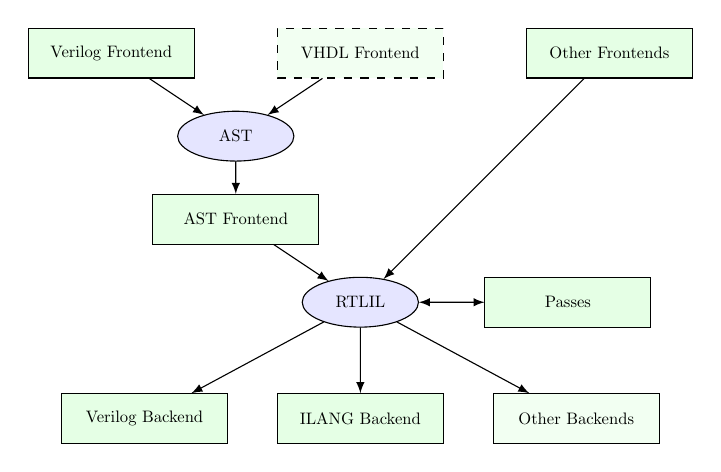
\begin{tikzpicture}[scale=0.6, every node/.style={transform shape}]
	\tikzstyle{process} = [draw, fill=green!10, rectangle, minimum height=3em, minimum width=10em, node distance=15em]
	\tikzstyle{data} = [draw, fill=blue!10, ellipse, minimum height=3em, minimum width=7em, node distance=15em]
	\node[process] (vlog) {Verilog Frontend};
	\node[process, dashed, fill=green!5] (vhdl) [right of=vlog] {VHDL Frontend};
	\node[process] (ilang) [right of=vhdl] {Other Frontends};
	\node[data] (ast) [below of=vlog, node distance=5em, xshift=7.5em] {AST};
	\node[process] (astfe) [below of=ast, node distance=5em] {AST Frontend};
	\node[data] (rtlil) [below of=astfe, node distance=5em, xshift=7.5em] {RTLIL};
	\node[process] (pass) [right of=rtlil, node distance=5em, xshift=7.5em] {Passes};
	\node[process] (vlbe) [below of=rtlil, node distance=7em, xshift=-13em] {Verilog Backend};
	\node[process] (ilangbe) [below of=rtlil, node distance=7em, xshift=0em] {ILANG Backend};
	\node[process, fill=green!5] (otherbe) [below of=rtlil, node distance=7em, xshift=+13em] {Other Backends};

	\draw[-latex] (vlog) -- (ast);
	\draw[-latex] (vhdl) -- (ast);
	\draw[-latex] (ast) -- (astfe);
	\draw[-latex] (astfe) -- (rtlil);
	\draw[-latex] (ilang) -- (rtlil);
	\draw[latex-latex] (rtlil) -- (pass);
	\draw[-latex] (rtlil) -- (vlbe);
	\draw[-latex] (rtlil) -- (ilangbe);
	\draw[-latex] (rtlil) -- (otherbe);
\end{tikzpicture}
\end{center}
\end{frame}

%%%%%%%%%%%%%%%%%%%%%%%%%%%%%%%%%%%%%%%%%%%%%%%%%%%%%%%%%%%%%%%%%%%%%%%%%%%%%

\subsection{Simplified RTLIL Entity-Relationship Diagram}

\begin{frame}{\subsecname}
Between passses and frontends/backends the design is stored in Yosys' internal
RTLIL (RTL Intermediate Language) format. For writing Yosys extensions it is
key to understand this format.

\bigskip
\begin{center}
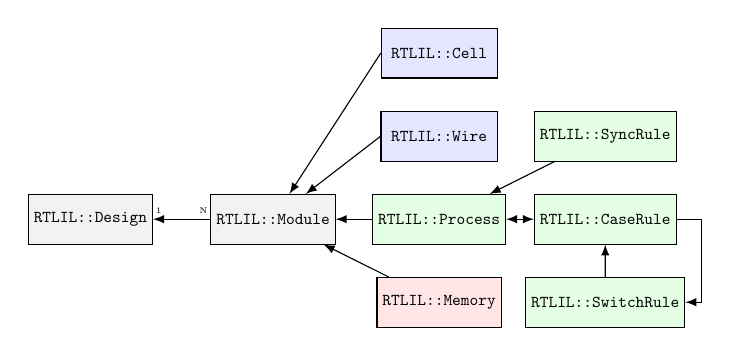
\begin{tikzpicture}[scale=0.6, every node/.style={transform shape}]
	\tikzstyle{entity} = [draw, fill=gray!10, rectangle, minimum height=3em, minimum width=7em, node distance=5em, font={\ttfamily}]
	\node[entity] (design) {RTLIL::Design};
	\node[entity] (module) [right of=design, node distance=11em] {RTLIL::Module} edge [-latex] node[above] {\tiny 1 \hskip3em N} (design);

	\node[entity] (process) [fill=green!10, right of=module, node distance=10em] {RTLIL::Process} (process.west) edge [-latex] (module);
	\node[entity] (memory) [fill=red!10, below of=process] {RTLIL::Memory} edge [-latex] (module);
	\node[entity] (wire) [fill=blue!10, above of=process] {RTLIL::Wire} (wire.west) edge [-latex] (module);
	\node[entity] (cell) [fill=blue!10, above of=wire] {RTLIL::Cell} (cell.west) edge [-latex] (module);

	\node[entity] (case) [fill=green!10, right of=process, node distance=10em] {RTLIL::CaseRule} edge [latex-latex] (process);
	\node[entity] (sync) [fill=green!10, above of=case] {RTLIL::SyncRule} edge [-latex] (process);
	\node[entity] (switch) [fill=green!10, below of=case] {RTLIL::SwitchRule} edge [-latex] (case);
	\draw[latex-] (switch.east) -- ++(1em,0) |- (case.east);
\end{tikzpicture}
\end{center}
\end{frame}

%%%%%%%%%%%%%%%%%%%%%%%%%%%%%%%%%%%%%%%%%%%%%%%%%%%%%%%%%%%%%%%%%%%%%%%%%%%%%

\subsection{RTLIL without memories and processes}

\begin{frame}[fragile]{\subsecname}
After the commands {\tt proc} and {\tt memory} (or {\tt memory -nomap}), we are
left with a much simpler version of RTLIL:

\begin{center}
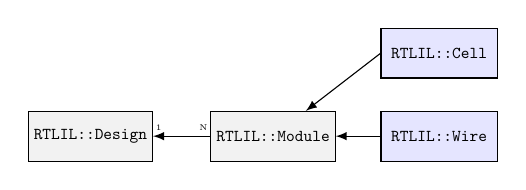
\begin{tikzpicture}[scale=0.6, every node/.style={transform shape}]
	\tikzstyle{entity} = [draw, fill=gray!10, rectangle, minimum height=3em, minimum width=7em, node distance=5em, font={\ttfamily}]
	\node[entity] (design) {RTLIL::Design};
	\node[entity] (module) [right of=design, node distance=11em] {RTLIL::Module} edge [-latex] node[above] {\tiny 1 \hskip3em N} (design);

	\node[entity] (wire) [fill=blue!10, right of=module, node distance=10em] {RTLIL::Wire} (wire.west) edge [-latex] (module);
	\node[entity] (cell) [fill=blue!10, above of=wire] {RTLIL::Cell} (cell.west) edge [-latex] (module);
\end{tikzpicture}
\end{center}

\bigskip
Many commands simply choose to only work on this simpler version:
\begin{lstlisting}[xleftmargin=0.5cm, basicstyle=\ttfamily\fontsize{8pt}{10pt}\selectfont]
if (module->processes.size() != 0 || module->memories.size() != 0)
    log_error("This command does not operate on modules with processes "
              "and/or memories! Run 'proc' and 'memory' first.\n");
\end{lstlisting}

\bigskip
For simplicity we only discuss this version of RTLIL in this presentation.
\end{frame}

%%%%%%%%%%%%%%%%%%%%%%%%%%%%%%%%%%%%%%%%%%%%%%%%%%%%%%%%%%%%%%%%%%%%%%%%%%%%%

\subsection{Using dump and show commands}

\begin{frame}{\subsecname}
\begin{itemize}
\item The {\tt dump} command prints the design (or parts of it) in ILANG format. This is
a text representation of RTLIL.

\bigskip
\item The {\tt show} command visualizes how the components in the design are connected.
\end{itemize}

\bigskip
When trying to understand what a command does, create a small test case and
look at the output of {\tt dump} and {\tt show} before and after the command
has been executed.
\end{frame}

%%%%%%%%%%%%%%%%%%%%%%%%%%%%%%%%%%%%%%%%%%%%%%%%%%%%%%%%%%%%%%%%%%%%%%%%%%%%%

\subsection{The RTLIL Data Structures}

\begin{frame}{\subsecname}
The RTLIL data structures are simple structs utilizing C++ {\tt std::}
containers.

\bigskip
\begin{itemize}
\item Most operations are performed directly on the RTLIL structs without
setter or getter functions.

\bigskip
\item In debug builds a consistency checker is run over the in-memory design
between commands to make sure that the RTLIL representation is intact.

\bigskip
\item Most RTLIL structs have helper methods that perform the most common operations.
\end{itemize}

\bigskip
See {\tt yosys/kernel/rtlil.h} for details.
\end{frame}

\subsubsection{RTLIL::IdString}

\begin{frame}{\subsubsecname}{}
{\tt RTLIL::IdString} is a simple wrapper for {\tt std::string}. It is used for names of RTLIL objects.

\medskip
The first character of a {\tt RTLIL::IdString} specifies if the name is {\it public\/} or {\it private\/}:

\medskip
\begin{itemize}
\item {\tt RTLIL::IdString[0] == '\textbackslash\textbackslash'}: \\
This is a public name. Usually this means it is a name that was declared in a Verilog file.

\bigskip
\item {\tt RTLIL::IdString[0] == '\$'}: \\
This is a private name. It was assigned by Yosys.
\end{itemize}

\bigskip
Use the {\tt NEW\_ID} macro to create a new unique private name.
\end{frame}

\subsubsection{RTLIL::Design and RTLIL::Module}

\begin{frame}[t, fragile]{\subsubsecname}
The {\tt RTLIL::Design} and {\tt RTLIL::Module} structs are the top-level RTLIL
data structures.

Yosys always operates on one active design, but can hold many designs in memory.

\bigskip
\begin{lstlisting}[xleftmargin=1cm, basicstyle=\ttfamily\fontsize{8pt}{10pt}\selectfont, language=C++]
struct RTLIL::Design {
    std::map<RTLIL::IdString, RTLIL::Module*> modules;
    ...
};

struct RTLIL::Module {
    RTLIL::IdString name;
    std::map<RTLIL::IdString, RTLIL::Wire*> wires;
    std::map<RTLIL::IdString, RTLIL::Cell*> cells;
    std::vector<RTLIL::SigSig> connections;
    ...
};
\end{lstlisting}
\end{frame}

\subsubsection{The RTLIL::Wire Structure}

\begin{frame}[t, fragile]{\subsubsecname}
Each wire in the design is represented by a {\tt RTLIL::Wire} struct:

\medskip
\begin{lstlisting}[xleftmargin=1cm, basicstyle=\ttfamily\fontsize{8pt}{10pt}\selectfont, language=C++]
struct RTLIL::Wire {
    RTLIL::IdString name;
    int width, start_offset, port_id;
    bool port_input, port_output;
    ...
};
\end{lstlisting}

\medskip
\hfil\begin{tabular}{p{3cm}l}
{\tt width} \dotfill & The total number of bits. E.g. 10 for {\tt [9:0]}. \\
{\tt start\_offset} \dotfill & The lowest bit index. E.g. 3 for {\tt [5:3]}. \\
{\tt port\_id} \dotfill & Zero for non-ports. Positive index for ports. \\
{\tt port\_input} \dotfill & True for {\tt input} and {\tt inout} ports. \\
{\tt port\_output} \dotfill & True for {\tt output} and {\tt inout} ports. \\
\end{tabular}
\end{frame}

\subsubsection{RTLIL::State and RTLIL::Const}

\begin{frame}[t, fragile]{\subsubsecname}
The {\tt RTLIL::State} enum represents a simple 1-bit logic level:

\smallskip
\begin{lstlisting}[xleftmargin=1cm, basicstyle=\ttfamily\fontsize{8pt}{10pt}\selectfont, language=C++]
enum RTLIL::State {
    S0 = 0,
    S1 = 1,
    Sx = 2, // undefined value or conflict
    Sz = 3, // high-impedance / not-connected
    Sa = 4, // don't care (used only in cases)
    Sm = 5  // marker (used internally by some passes)
};
\end{lstlisting}

\bigskip
The {\tt RTLIL::Const} struct represents a constant multi-bit value:

\smallskip
\begin{lstlisting}[xleftmargin=1cm, basicstyle=\ttfamily\fontsize{8pt}{10pt}\selectfont, language=C++]
struct RTLIL::Const {
    std::vector<RTLIL::State> bits;
    ...
};
\end{lstlisting}

\bigskip
Notice that Yosys is not using special {\tt VCC} or {\tt GND} driver cells to represent constants. Instead
constants are part of the RTLIL representation itself.
\end{frame}

\subsubsection{The RTLIL::SigSpec Structure}

\begin{frame}[t, fragile]{\subsubsecname}
The {\tt RTLIL::SigSpec} struct represents a signal vector. Each bit can either be a bit from a wire
or a constant value. Consecutive bits from a wire or consecutive constant bits are consolidated into
a {\tt RTLIL::SigChunk}:

\bigskip
\begin{lstlisting}[xleftmargin=1cm, basicstyle=\ttfamily\fontsize{8pt}{10pt}\selectfont, language=C++]
struct RTLIL::SigChunk {
    RTLIL::Wire *wire;
    RTLIL::Const data; // only used if wire == NULL
    int width, offset;
    ...
};

struct RTLIL::SigSpec {
    std::vector<RTLIL::SigChunk> chunks; // LSB at index 0
    int width;
    ...
};
\end{lstlisting}

\bigskip
The {\tt RTLIL::SigSpec} struct has a ton of additional helper methods to compare, analyze, and
manipulate instances of {\tt RTLIL::SigSpec}.
\end{frame}

\subsubsection{The RTLIL::Cell Structure}

\begin{frame}[t, fragile]{\subsubsecname (1/2)}
The {\tt RTLIL::Cell} struct represents an instance of a module or library cell.

\smallskip
The ports of the cell
are associated with {\tt RTLIL::SigSpec} instances and the parameters are associated with {\tt RTLIL::Const}
instances:

\bigskip
\begin{lstlisting}[xleftmargin=1cm, basicstyle=\ttfamily\fontsize{8pt}{10pt}\selectfont, language=C++]
struct RTLIL::Cell {
    RTLIL::IdString name, type;
    std::map<RTLIL::IdString, RTLIL::SigSpec> connections;
    std::map<RTLIL::IdString, RTLIL::Const> parameters;
    ...
};
\end{lstlisting}

\bigskip
The {\tt type} may refer to another module in the same design, a cell name from a cell library, or a
cell name from the internal cell library:

\begin{lstlisting}[xleftmargin=1cm, basicstyle=\ttfamily\fontsize{6pt}{7pt}\selectfont]
$not $pos $bu0 $neg $and $or $xor $xnor $reduce_and $reduce_or $reduce_xor $reduce_xnor
$reduce_bool $shl $shr $sshl $sshr $lt $le $eq $ne $eqx $nex $ge $gt $add $sub $mul $div $mod
$pow $logic_not $logic_and $logic_or $mux $pmux $slice $concat $lut $assert $sr $dff
$dffsr $adff $dlatch $dlatchsr $memrd $memwr $mem $fsm $_NOT_ $_AND_ $_OR_ $_XOR_ $_MUX_ $_SR_NN_
$_SR_NP_ $_SR_PN_ $_SR_PP_ $_DFF_N_ $_DFF_P_ $_DFF_NN0_ $_DFF_NN1_ $_DFF_NP0_ $_DFF_NP1_ $_DFF_PN0_
$_DFF_PN1_ $_DFF_PP0_ $_DFF_PP1_ $_DFFSR_NNN_ $_DFFSR_NNP_ $_DFFSR_NPN_ $_DFFSR_NPP_ $_DFFSR_PNN_
$_DFFSR_PNP_ $_DFFSR_PPN_ $_DFFSR_PPP_ $_DLATCH_N_ $_DLATCH_P_ $_DLATCHSR_NNN_ $_DLATCHSR_NNP_
$_DLATCHSR_NPN_ $_DLATCHSR_NPP_ $_DLATCHSR_PNN_ $_DLATCHSR_PNP_ $_DLATCHSR_PPN_ $_DLATCHSR_PPP_
\end{lstlisting}
\end{frame}

\begin{frame}[t, fragile]{\subsubsecname (2/2)}
Simulation models (i.e. {\it documentation\/} :-) for the internal cell library:

\smallskip
\hskip2em {\tt yosys/techlibs/common/simlib.v} and \\
\hskip2em {\tt yosys/techlibs/common/simcells.v}

\bigskip
The lower-case cell types (such as {\tt \$and}) are parameterized cells of variable
width. This so-called {\it RTL Cells\/} are the cells described in {\tt simlib.v}. 

\bigskip
The upper-case cell types (such as {\tt \$\_AND\_}) are single-bit cells that are not
parameterized. This so-called {\it Internal Logic Gates} are the cells described
in {\tt simcells.v}.

\bigskip
The consistency checker also checks the interfaces to the internal cell library.
If you want to use private cell types for your own purposes, use the {\tt \$\_\_}-prefix
to avoid name collisions.
\end{frame}

\subsubsection{Connecting wires or constant drivers}

\begin{frame}[t, fragile]{\subsubsecname}
Additional connections between wires or between wires and constants are modelled using
{\tt RTLIL::Module::connections}:

\bigskip
\begin{lstlisting}[xleftmargin=1cm, basicstyle=\ttfamily\fontsize{8pt}{10pt}\selectfont, language=C++]
typedef std::pair<RTLIL::SigSpec, RTLIL::SigSpec> RTLIL::SigSig;

struct RTLIL::Module {
    ...
    std::vector<RTLIL::SigSig> connections;
    ...
};
\end{lstlisting}

\bigskip
{\tt RTLIL::SigSig::first} is the driven signal and {\tt RTLIL::SigSig::second} is the driving signal.
Example usage (setting wire {\tt foo} to value {\tt 42}):
\begin{lstlisting}[xleftmargin=1cm, basicstyle=\ttfamily\fontsize{8pt}{10pt}\selectfont, language=C++]
module->connections.push_back(RTLIL::SigSig(module->wires.at("\\foo"),
        RTLIL::SigSpec(42, module->wires.at("\\foo")->width)));
\end{lstlisting}
\end{frame}

%%%%%%%%%%%%%%%%%%%%%%%%%%%%%%%%%%%%%%%%%%%%%%%%%%%%%%%%%%%%%%%%%%%%%%%%%%%%%

\subsection{Creating modules from scratch}

\begin{frame}[t, fragile]{\subsecname}
Let's create the following module using the RTLIL API:

\smallskip
\begin{lstlisting}[xleftmargin=1cm, basicstyle=\ttfamily\fontsize{8pt}{10pt}\selectfont, language=Verilog]
module absval(input signed [3:0] a, output [3:0] y);
    assign y = a[3] ? -a : a;
endmodule
\end{lstlisting}

\smallskip
\begin{lstlisting}[xleftmargin=1cm, basicstyle=\ttfamily\fontsize{8pt}{10pt}\selectfont, language=C++]
RTLIL::Module *module = new RTLIL::Module;
module->name = "\\absval";

RTLIL::Wire *a = module->new_wire(4, "\\a");
a->port_input = true;
a->port_id = 1;

RTLIL::Wire *y = module->new_wire(4, "\\y");
y->port_output = true;
y->port_id = 2;

RTLIL::Wire *a_inv = module->new_wire(4, NEW_ID);
module->addNeg(NEW_ID, a, a_inv, true);
module->addMux(NEW_ID, a, a_inv, RTLIL::SigSpec(a, 1, 3), y);
\end{lstlisting}
\end{frame}

%%%%%%%%%%%%%%%%%%%%%%%%%%%%%%%%%%%%%%%%%%%%%%%%%%%%%%%%%%%%%%%%%%%%%%%%%%%%%

\subsection{Modifying modules}

\begin{frame}{\subsecname}
Most commands modify existing modules, not create new ones.

When modifying existing modules, stick to the following DOs and DON'Ts:

\begin{itemize}
\item Do not remove wires. Simply disconnect them and let a successive {\tt clean} command worry about removing it.

\item Use {\tt module->fixup\_ports()} after changing the {\tt port\_*} properties of wires.

\item You can safely remove cells or change the {\tt connetions} property of a cell, but be careful when
changing the size of the {\tt SigSpec} connected to a cell port.

\item Use the {\tt SigMap} helper class (see next slide) when you need a unique handle for each signal bit.
\end{itemize}
\end{frame}

%%%%%%%%%%%%%%%%%%%%%%%%%%%%%%%%%%%%%%%%%%%%%%%%%%%%%%%%%%%%%%%%%%%%%%%%%%%%%

\subsection{Using the SigMap helper class}

\begin{frame}[t, fragile]{\subsecname}
Consider the following module:

\smallskip
\begin{lstlisting}[xleftmargin=1cm, basicstyle=\ttfamily\fontsize{8pt}{10pt}\selectfont, language=Verilog]
module test(input a, output x, y);
    assign x = a, y = a;
endmodule
\end{lstlisting}

In this case {\tt a}, {\tt x}, and {\tt y} are all different names for the same signal. However:

\smallskip
\begin{lstlisting}[xleftmargin=1cm, basicstyle=\ttfamily\fontsize{8pt}{10pt}\selectfont, language=C++]
RTLIL::SigSpec a(module->wires.at("\\a")), x(module->wires.at("\\x")),
                                           y(module->wires.at("\\y"));
log("%d %d %d\n", a == x, x == y, y == a); // will print "0 0 0"
\end{lstlisting}

The {\tt SigMap} helper class can be used to map all such aliasing signals to a
unique signal from the group (usually the wire that is directly driven by a cell or port).

\smallskip
\begin{lstlisting}[xleftmargin=1cm, basicstyle=\ttfamily\fontsize{8pt}{10pt}\selectfont, language=C++]
SigMap sigmap(module);
log("%d %d %d\n", sigmap(a) == sigmap(x), sigmap(x) == sigmap(y),
                  sigmap(y) == sigmap(a)); // will print "1 1 1"
\end{lstlisting}
\end{frame}

%%%%%%%%%%%%%%%%%%%%%%%%%%%%%%%%%%%%%%%%%%%%%%%%%%%%%%%%%%%%%%%%%%%%%%%%%%%%%

\subsection{Printing log messages}

\begin{frame}[t, fragile]{\subsecname}
The {\tt log()} function is a {\tt printf()}-like function that can be used to create log messages.

\medskip
Use {\tt log\_signal()} to create a C-string for a SigSpec object\footnote[frame]{The pointer returned
by {\tt log\_signal()} is automatically freed by the log framework at a later time.}:
\begin{lstlisting}[xleftmargin=1cm, basicstyle=\ttfamily\fontsize{8pt}{10pt}\selectfont, language=C++]
log("Mapped signal x: %s\n", log_signal(sigmap(x)));
\end{lstlisting}

\medskip
Use {\tt RTLIL::id2cstr()} to create a C-string for an {\tt RTLIL::IdString}:
\begin{lstlisting}[xleftmargin=1cm, basicstyle=\ttfamily\fontsize{8pt}{10pt}\selectfont, language=C++]
log("Name of this module: %s\n", RTLIL::id2cstr(module->name));
\end{lstlisting}

\medskip
Use {\tt log\_header()} and {\tt log\_push()}/{\tt log\_pop()} to structure log messages:
\begin{lstlisting}[xleftmargin=1cm, basicstyle=\ttfamily\fontsize{8pt}{10pt}\selectfont, language=C++]
log_header("Doing important stuff!\n");
log_push();
for (int i = 0; i < 10; i++)
    log("Log message #%d.\n", i);
log_pop();
\end{lstlisting}
\end{frame}

%%%%%%%%%%%%%%%%%%%%%%%%%%%%%%%%%%%%%%%%%%%%%%%%%%%%%%%%%%%%%%%%%%%%%%%%%%%%%

\subsection{Error handling}

\begin{frame}[t, fragile]{\subsecname}
Use {\tt log\_error()} to report a non-recoverable error:

\medskip
\begin{lstlisting}[xleftmargin=1cm, basicstyle=\ttfamily\fontsize{8pt}{10pt}\selectfont, language=C++]
if (design->modules.count(module->name) != 0)
    log_error("A module with the name %s already exists!\n",
            RTLIL::id2cstr(module->name));
\end{lstlisting}

\bigskip
Use {\tt log\_cmd\_error()} to report a recoverable error:
\begin{lstlisting}[xleftmargin=1cm, basicstyle=\ttfamily\fontsize{8pt}{10pt}\selectfont, language=C++]
if (design->selection_stack.back().empty())
    log_cmd_error("This command can't operator on an empty selection!\n");
\end{lstlisting}

\bigskip
Use {\tt log\_assert()} and {\tt log\_abort()} instead of {\tt assert()} and {\tt abort()}.
\end{frame}

%%%%%%%%%%%%%%%%%%%%%%%%%%%%%%%%%%%%%%%%%%%%%%%%%%%%%%%%%%%%%%%%%%%%%%%%%%%%%

\subsection{Creating a command}

\begin{frame}[t, fragile]{\subsecname}
Simply create a global instance of a class derived from {\tt Pass} to create
a new yosys command:

\bigskip
\begin{lstlisting}[xleftmargin=1cm, basicstyle=\ttfamily\fontsize{8pt}{10pt}\selectfont, language=C++]
#include "kernel/rtlil.h"
#include "kernel/register.h"
#include "kernel/log.h"

struct MyPass : public Pass {
    MyPass() : Pass("my_cmd", "just a simple test") { }
    virtual void execute(std::vector<std::string> args, RTLIL::Design *design)
    {
        log("Arguments to my_cmd:\n");
        for (auto &arg : args)
            log("  %s\n", arg.c_str());

        log("Modules in current design:\n");
        for (auto &mod : design->modules)
            log("  %s (%zd wires, %zd cells)\n", RTLIL::id2cstr(mod.first),
                    mod.second->wires.size(), mod.second->cells.size());
    }
} MyPass;
\end{lstlisting}
\end{frame}

%%%%%%%%%%%%%%%%%%%%%%%%%%%%%%%%%%%%%%%%%%%%%%%%%%%%%%%%%%%%%%%%%%%%%%%%%%%%%

\subsection{Creating a plugin}

\begin{frame}[fragile]{\subsecname}
Yosys can be extended by adding additional C++ code to the Yosys code base, or
by loading plugins into Yosys.

\bigskip
Use the following command to compile a Yosys plugin:
\begin{lstlisting}[xleftmargin=1cm, basicstyle=\ttfamily\fontsize{8pt}{10pt}\selectfont]
yosys-config --exec --cxx --cxxflags --ldflags \
             -o my_cmd.so -shared my_cmd.cc --ldlibs
\end{lstlisting}

\bigskip
Load the plugin using the yosys {\tt -m} option:
\begin{lstlisting}[xleftmargin=1cm, basicstyle=\ttfamily\fontsize{8pt}{10pt}\selectfont]
yosys -m ./my_cmd.so -p 'my_cmd foo bar'
\end{lstlisting}
\end{frame}

%%%%%%%%%%%%%%%%%%%%%%%%%%%%%%%%%%%%%%%%%%%%%%%%%%%%%%%%%%%%%%%%%%%%%%%%%%%%%

\subsection{Summary}

\begin{frame}{\subsecname}
\begin{itemize}
\item Writing Yosys extensions is very straight-forward.
\item \dots and even simpler if you don't need RTLIL::Memory or RTLIL::Process objects.

\bigskip
\item Writing synthesis software? Consider learning the Yosys API and make your stuff
part of the Yosys framework.
\end{itemize}

\bigskip
\bigskip
\begin{center}
Questions?
\end{center}

\bigskip
\bigskip
\begin{center}
\url{http://www.clifford.at/yosys/}
\end{center}
\end{frame}



\end{document}
